\graphicspath{{Figures/}}

\title{\fontsize{33}{45}{\huge Pattern Classification (EET 3035)\newline \vspace{8pt} \Large Lecture 06\vspace{-1.1cm}}}
\author{\vspace{-0.4cm}\\\normalsize{\bf Dr. Kundan Kumar}\\ PhD (IIT Kharagpur)\\
Associate Professor\\Department of ECE}
% - Give the names in the same order as the appear in the paper.
% - Use the \inst{?} command only if the authors have different
%   affiliation.

\institute[Indian Institute of Technology Kharagpur] % (optional, but mostly needed)
{
\includegraphics[height=.17\textheight]{SOAlogo.png}\\
 Faculty of Engineering (ITER)\\ S`O'A Deemed to be University, Bhubaneswar, India-751030\\
 \copyright\  2019 Kundan Kumar, All Rights Reserved\\
  \vspace{-1.1cm}}
% - Use the \inst command only if there are several affiliations.
% - Keep it simple, no one is interested in your street address.
\date{}
% To remove page number from a perticular slide
{
\setbeamertemplate{logo}{}
\makeatletter
\setbeamertemplate{footline}{
        \leavevmode%
  
  % First line.
  \hbox{%
  \begin{beamercolorbox}[wd=.2\paperwidth,ht=\beamer@decolines@lineup,dp=0pt]{}%
  \end{beamercolorbox}%
  \begin{beamercolorbox}[wd=.8\paperwidth,ht=\beamer@decolines@lineup,dp=0pt]{lineup}%
  \end{beamercolorbox}%
  } %
  % Second line.
  \hbox{%
  \begin{beamercolorbox}[wd=\paperwidth,ht=\beamer@decolines@linemid,dp=0pt]{linemid}%
  \end{beamercolorbox}%
  } %
  % Third line.
  \hbox{%
  \begin{beamercolorbox}[wd=.1\paperwidth,ht=\beamer@decolines@linebottom,dp=0pt]{}%
  \end{beamercolorbox}%
  \begin{beamercolorbox}[wd=.9\paperwidth,ht=\beamer@decolines@linebottom,dp=0pt]{linebottom}%
  \end{beamercolorbox}%
  }%
        }
\makeatother
\begin{frame}
\titlepage
\end{frame}
}

\section{Linear Discriminant Functions}
\subsection{}
\begin{frame}{}
\begin{variableblock}{\centering \Large \textbf{\vspace{4pt}\newline Linear Discriminant Functions\vspace{4pt}}}{bg=slidecolor,fg=white}{bg=slidecolor,fg=white}
\end{variableblock}
\end{frame}

\begin{frame}{Linear discriminant functions and decisions surfaces}
\begin{itemize}
\item A {\color{mycolor1}discriminant function} is a linear combination of the components of ${\rm x}$ can be written as
\begin{equation}
g(x)={\rm w}^T{\rm x}+w_0 \nonumber
\end{equation}
where ${\rm w}$ is the {\color{mycolor2}weight vector} and $w_0$ the {\color{mycolor4}bias} or {\color{mycolor4}threshold} weight.
\item The equation $g({\rm x}) = 0$ defines the {\color{mycolor1}decision surface} that separates points from different classes.
\item Linear discriminant functions are going to be studied for 
\begin{itemize}
\item two-category case,
\item multi-category case, and
\item general case
\end{itemize} 
For the general case
there will be $c$ such discriminant functions, one for each of $c$ categories.\nocite{duda2012pattern}
%\item A two-category classifier with a discriminant function of the form (1) uses the following rule:\\
%	Decide $w_1$ if $g(x) > 0$ and $w_2$ if $g(x) < 0$\\
%	Decide $w_1$ if ${\rm w}^tx > -w_0$ and $w_2$ otherwise\\
%	If $g(x) = 0$ then $x$ is assigned to either class
\end{itemize}
\end{frame}

\section{Two-category}
\subsection{}
\begin{frame}{Two-Category Case}
\begin{itemize}
\setlength{\itemsep}{12pt}
\item A two-category classifier with a discriminant function of the form $g({\rm x})={\rm w}^T{\rm x}+w_0$ uses the following rule:\\
\begin{equation}
{\sf Decide}~~~~\left\{ {\begin{array}{*{20}{c}}
{{\omega_1}}&{{\sf if}~g({\rm x}) > 0}\\
{{\omega_2}}&{\rm otherwise}
\end{array}} \right.\nonumber
\end{equation}
\item Thus, ${\rm x}$ is assigned to $\omega_1$ if the {\color{mycolor2}inner product} ${\rm w}^T{\rm x}$ exceeds the
threshold $-w_0$ and to $\omega_2$ otherwise.
\item If $g({\rm x})=0$, ${\rm x}$ can ordinarily be assigned to either class, or can be left undefined.
\begin{equation}
{\sf Decide}~~~~\left\{ {\begin{array}{*{20}{c}}
{{\omega_1}}&{{\sf if}~g({\rm x}) \geq 0}\\
{{\omega_2}}&{\rm otherwise}
\end{array}} \right.\nonumber
\end{equation}
\end{itemize}
\end{frame}

\begin{frame}{A simple linear classifier}
\begin{figure}
\includegraphics[scale=0.93]{Ch0501}
\caption{A simple linear classifier having $d$ input units, each corresponding to the values of the components of an input vector. Each input feature value $x_i$ is multiplied by its corresponding weight $w_i$; the output unit sums all these products and emits $+1$ if ${\rm w}^T{\rm x}+w_0>0$ or $-1$ otherwise}
\end{figure}
\end{frame}

\begin{frame}{Two-Category Case}
\begin{itemize}
\item The equation $g({\rm x}) = 0$ defines the decision surface that separates points assigned to the category ${\omega_1}$ from points assigned to the category ${\omega}_2$
\item When $g({\rm x})$ is linear, the decision surface is a hyperplane.
%\item Algebraic measure of the distance from ${\rm x}$ to the hyperplane (interesting result!)
\item If ${\rm x}_1$ and ${\rm x}_2$ are both on the decision
surface, then
\begin{align}
{\rm w}^T{\rm x}_1+w_0={\rm w}^T{\rm x}_2+w_0 \nonumber\\
\Rightarrow ~~~~{\rm w}^T({\rm x}_1-{\rm x}_2)=0\nonumber
\end{align}
\item This shows that ${\rm w}$ is normal to any vector lying in the hyperplane.
\end{itemize}
\end{frame}

\begin{frame}{Two-Category Case}
\begin{itemize}
\item The discriminant function $g({\rm x})$ gives an algebraic measure of the distance from $\rm x$ to the hyperplane. The easiest way to see this is to express ${\rm x}$ as
\begin{equation}
{\rm x} = {{\rm x}_p} + r\frac{{\rm w}}{{\left\| {\rm w} \right\|}} \nonumber
\end{equation}
\end{itemize}
\begin{columns}
\begin{column}{6.5cm}
\begin{itemize}
\item where ${\rm x}_p$ is the normal projection of ${\rm x}$ onto $H$, and $r$ is the desired algebraic distance which is positive if ${\rm x}$ is on the positive side and negative if ${\rm x}$ is on the negative side.
\item Because, $g({\rm x}_p)=0$
\begin{equation}
r = \frac{{g({\rm x})}}{{\left\| {\rm w} \right\|}}~~~~~~~~~~~~~~~~~~~~~~~~~ \nonumber
\end{equation}
\end{itemize}
\end{column}
\begin{column}{4cm}
\vspace{-1cm}
\begin{figure}
\includegraphics[scale=0.95]{Ch0502}
\end{figure}
\end{column}
\end{columns}
\end{frame}

\begin{frame}{Two-Category Case}
\begin{itemize}
\item The distance from the origin to $H$ is given by $\frac{w_0}{||{\rm w}||}$. If $w_0>0$, the origin is on the positive side of $H$, and if $w_0<0$, it is on the negative side.
\end{itemize}
\begin{figure}
\includegraphics[scale=0.85]{Ch0502}
\caption{The linear decision boundary $H$, where $g(x)={\rm w}^T{\rm x}+w_0$, separates the feature space into two half-spaces $\mathcal{R}_1$ (where $g({\rm  x})>0$) and $\mathcal{R}_2$ (where $g({\rm x})<0)$)}
\end{figure}
\end{frame}

\begin{frame}{Two-Category Case}
\begin{itemize}
\item In conclusion, a linear discriminant function divides the feature space by a hyperplane decision surface.
\item The orientation of the surface is determined by the normal vector ${\rm w}$ and the location of the surface is determined by the bias $w_0$.
\item The discriminant function $g({\rm x})$ is proportional to the signed distance from ${\rm x}$ to the hyperplane, with $g({\rm x})>0$ when ${\rm x}$ is on the positive side, and $g({\rm x})<0$ when ${\rm x}$ is on the negative side.
\end{itemize}
\end{frame}

\section{Multi-category}
\subsection{}
\begin{frame}{Multi-category case}
\begin{itemize}
\item There is more than one way to devise multi-category classifiers employing linear discriminant functions.
\begin{columns}
\begin{column}{4cm}
\begin{itemize}
\item c two-class problem ({\color{mycolor1}one-vs-rest})
\end{itemize}
\begin{figure}
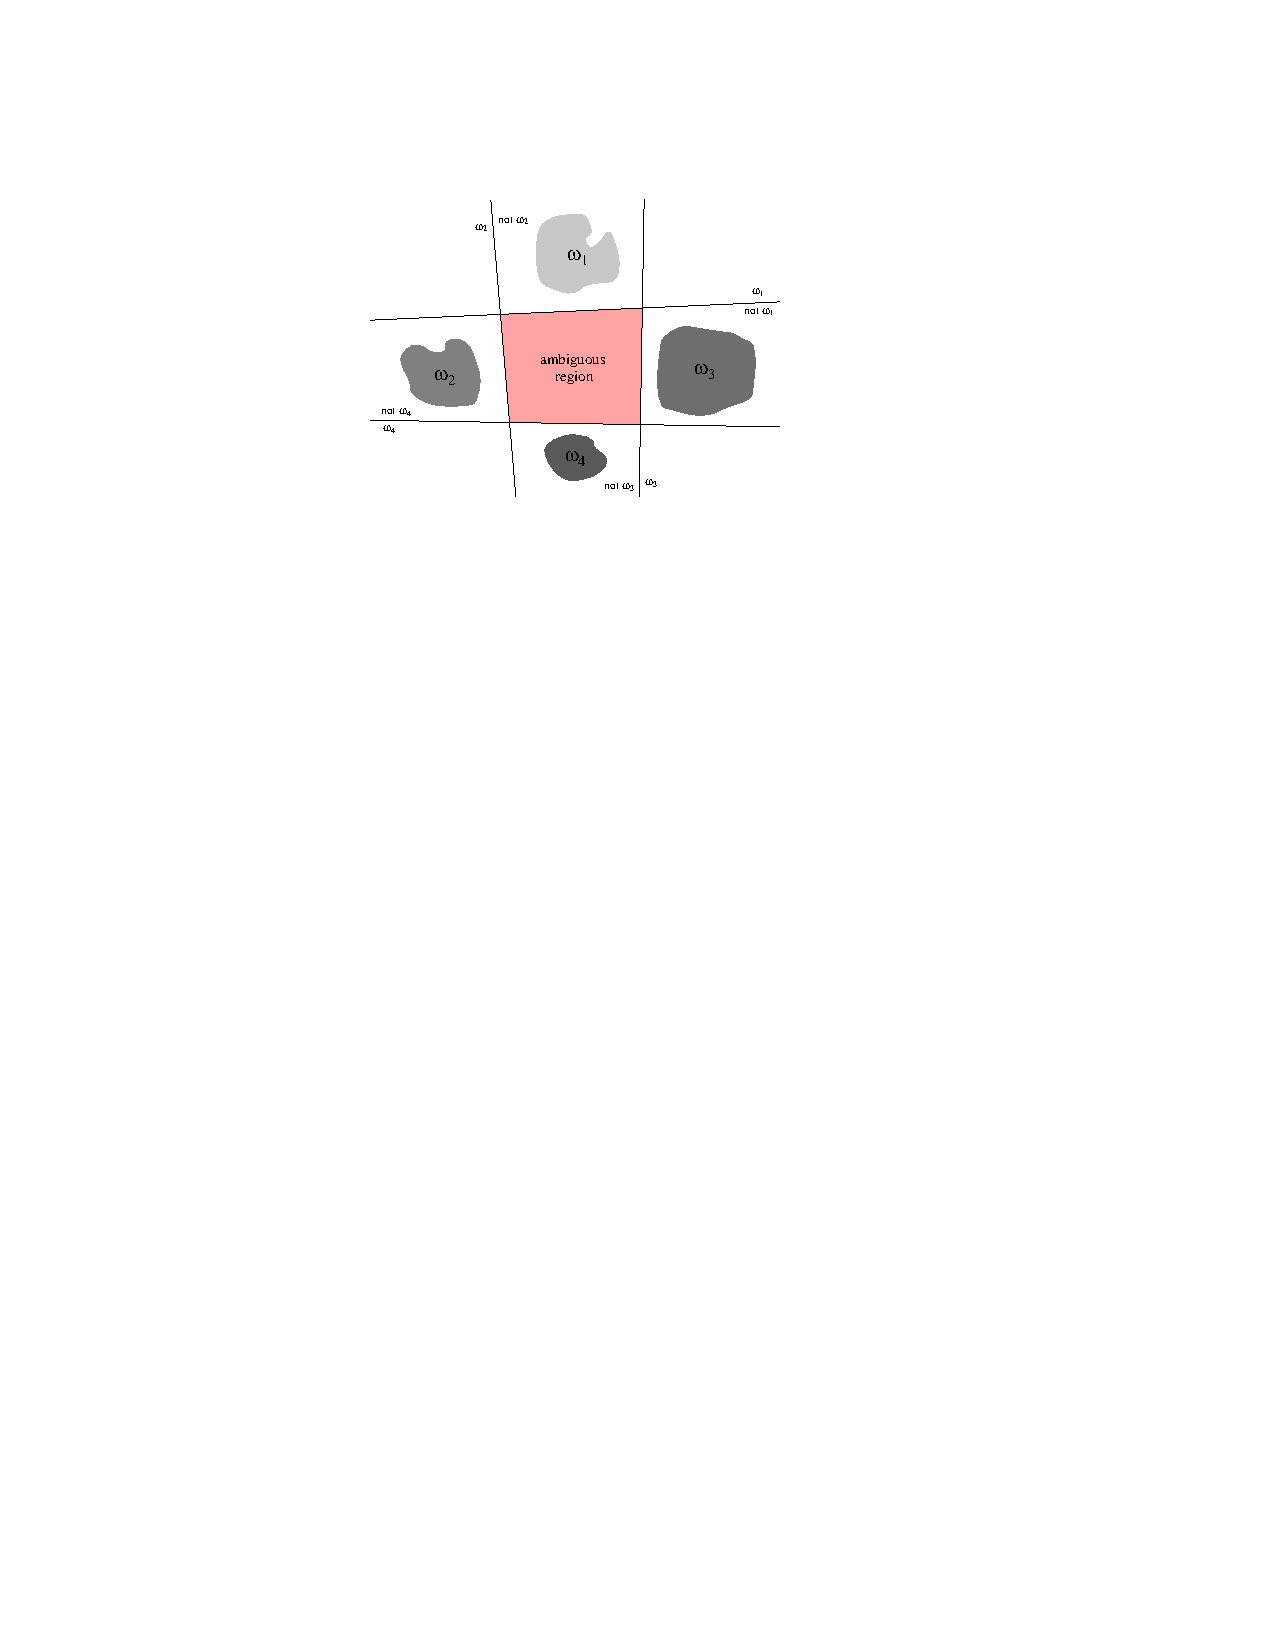
\includegraphics[scale=0.65]{ldf01}
\end{figure}
\end{column}
\begin{column}{5cm}
\begin{itemize}
\item $c(c-1)/2$ linear discriminants, one for every pair of classes ({\color{mycolor1}one-vs-one}).
\end{itemize}
\begin{figure}
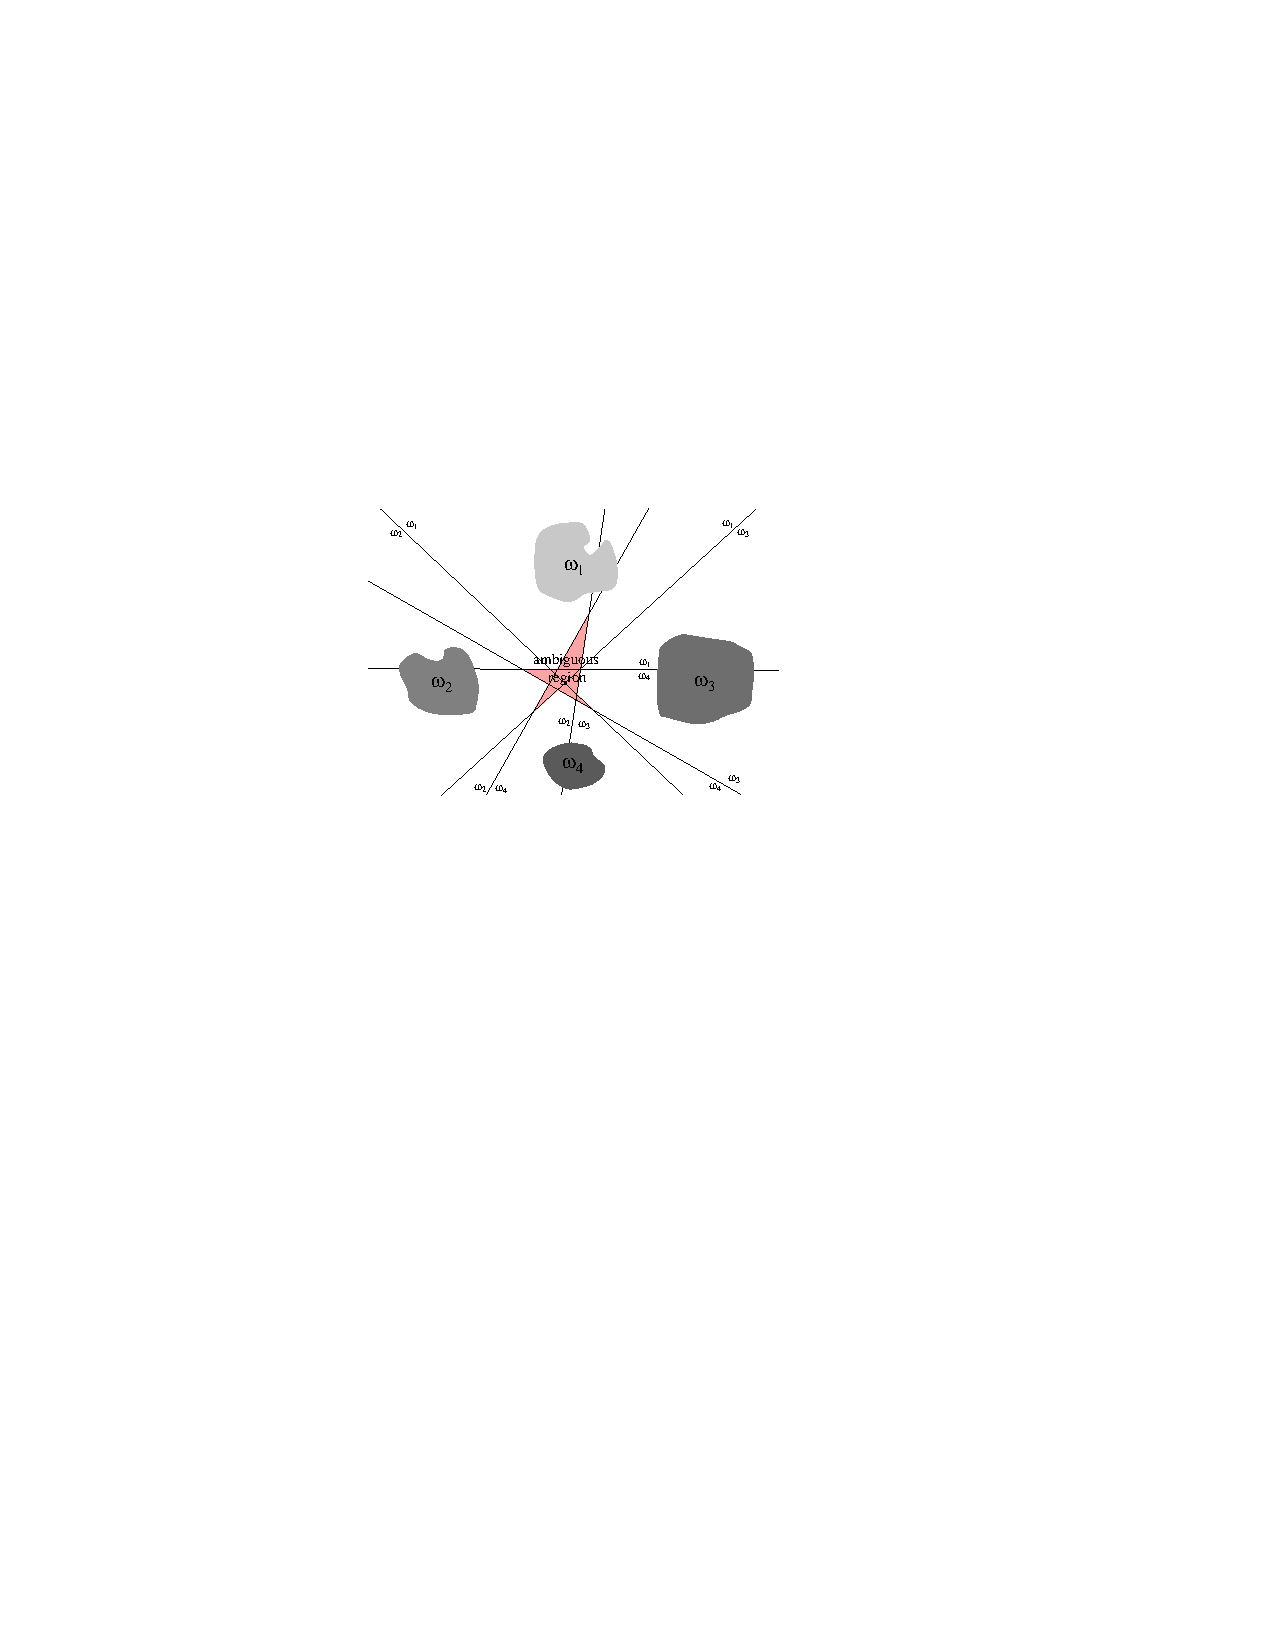
\includegraphics[scale=0.65]{ldf02}
\end{figure}
\end{column}
\end{columns}

\item Pink regions have ambiguous category assignment.
\end{itemize}
\end{frame}

\begin{frame}{Multi-category case}
\begin{itemize}
\item More effective way is to define $c$ linear discriminant functions
\begin{equation}
g_i({\rm x})={\rm w}^T_i{\rm x}+w_{i0}~~~~i=1,2,\ldots,c \nonumber
\end{equation}
	and assign ${\rm x}$ to $\omega_i$ if $g_i({\rm x}) > g_j({\rm x})$ for all $j\neq i$; in case of ties, the classification is undefined
\item In this case, resulting classifier is a ``\textit{\color{mycolor2}linear machine}''.
\item A linear machine divides the feature space into $c$ decision regions, with $g_i({\rm x})$ being the largest discriminant if ${\rm x}$ is in the region $\mathcal{R}_i$.
\item For a two contiguous regions $\mathcal{R}_i$ and $\mathcal{R}_j$; the boundary that separates them is a portion of hyperplane $H_{ij}$ defined by:
\begin{equation}
g_i({\rm x})=g_j({\rm x})~~~~~or~~~~~({\rm w}_i-{\rm w}_j)^T{\rm x}+(w_{i0}-w_{j0})=0 \nonumber
\end{equation}
\end{itemize}
\end{frame}

\begin{frame}{Multi-category case}
\begin{itemize}
\item It follows at once that ${\rm w}_i-{\rm w}_j$ is normal to $H_{ij}$, and the signed distance from ${\rm x}$ to $H_{ij}$ is given by 
\begin{equation}
r = \frac{{({g_i}({\rm x}) - {g_j}({\rm x}))}}{{\left\| {{{\rm w}_i} - {{\rm w}_j}} \right\|}} \nonumber
\end{equation}
\end{itemize}
\begin{figure}
\includegraphics[scale=0.7]{Ch0503}
\caption{Decision boundaries produced by a linear machine for a three-class problem and a five-class problem}
\end{figure}
\end{frame}



%\begin{frame}{The Two-Category Case}
%\begin{itemize}
%\item For the two-category case, the decision rule can be written as
%\begin{equation}
%{\sf Decide}~~~~\left\{ {\begin{array}{*{20}{c}}
%{{\omega_1}}&{{\sf if}~g({\rm x})>0}\\
%{{\omega_2}}&{\sf otherwise~~~~~~~}
%\end{array}} \right.\nonumber
%\end{equation}
%\item The equation $g({\rm x}) = 0$ defines the decision boundary that separates points assigned to $\omega_1$ from points assigned to $\omega_2$.
%\item When $g({\rm x})$ is linear, the decision surface is a hyperplane whose orientation is determined by the normal vector ${\rm w}$ and location is determined by the bias $w_0$.
%\end{itemize}
%\end{frame}

%\begin{frame}{The Multicategory Case}
%\begin{itemize}
%\item There is more than one way to devise multicategory classifiers using linear discriminant functions.
%\item For example, we can reduce the problem as $c$ two-class problems, where the $i$th problem is solved by a linear discriminant that separates points assigned to $\omega_i$ from those not assigned to $\omega_i$.
%\item Alternatively, we can use $c(c-1)/2$ linear discriminants, one for every pair of classes.
%\item Also, we can use $c$ linear discriminants, one for each class, and assign $x$ to $\omega_i$
%if $g_i({\rm x}) > g_j ({\rm x})$ for all $j\neq i$.
%\end{itemize}
%\end{frame}

%\begin{frame}{The Multicategory Case}
%\begin{figure}
%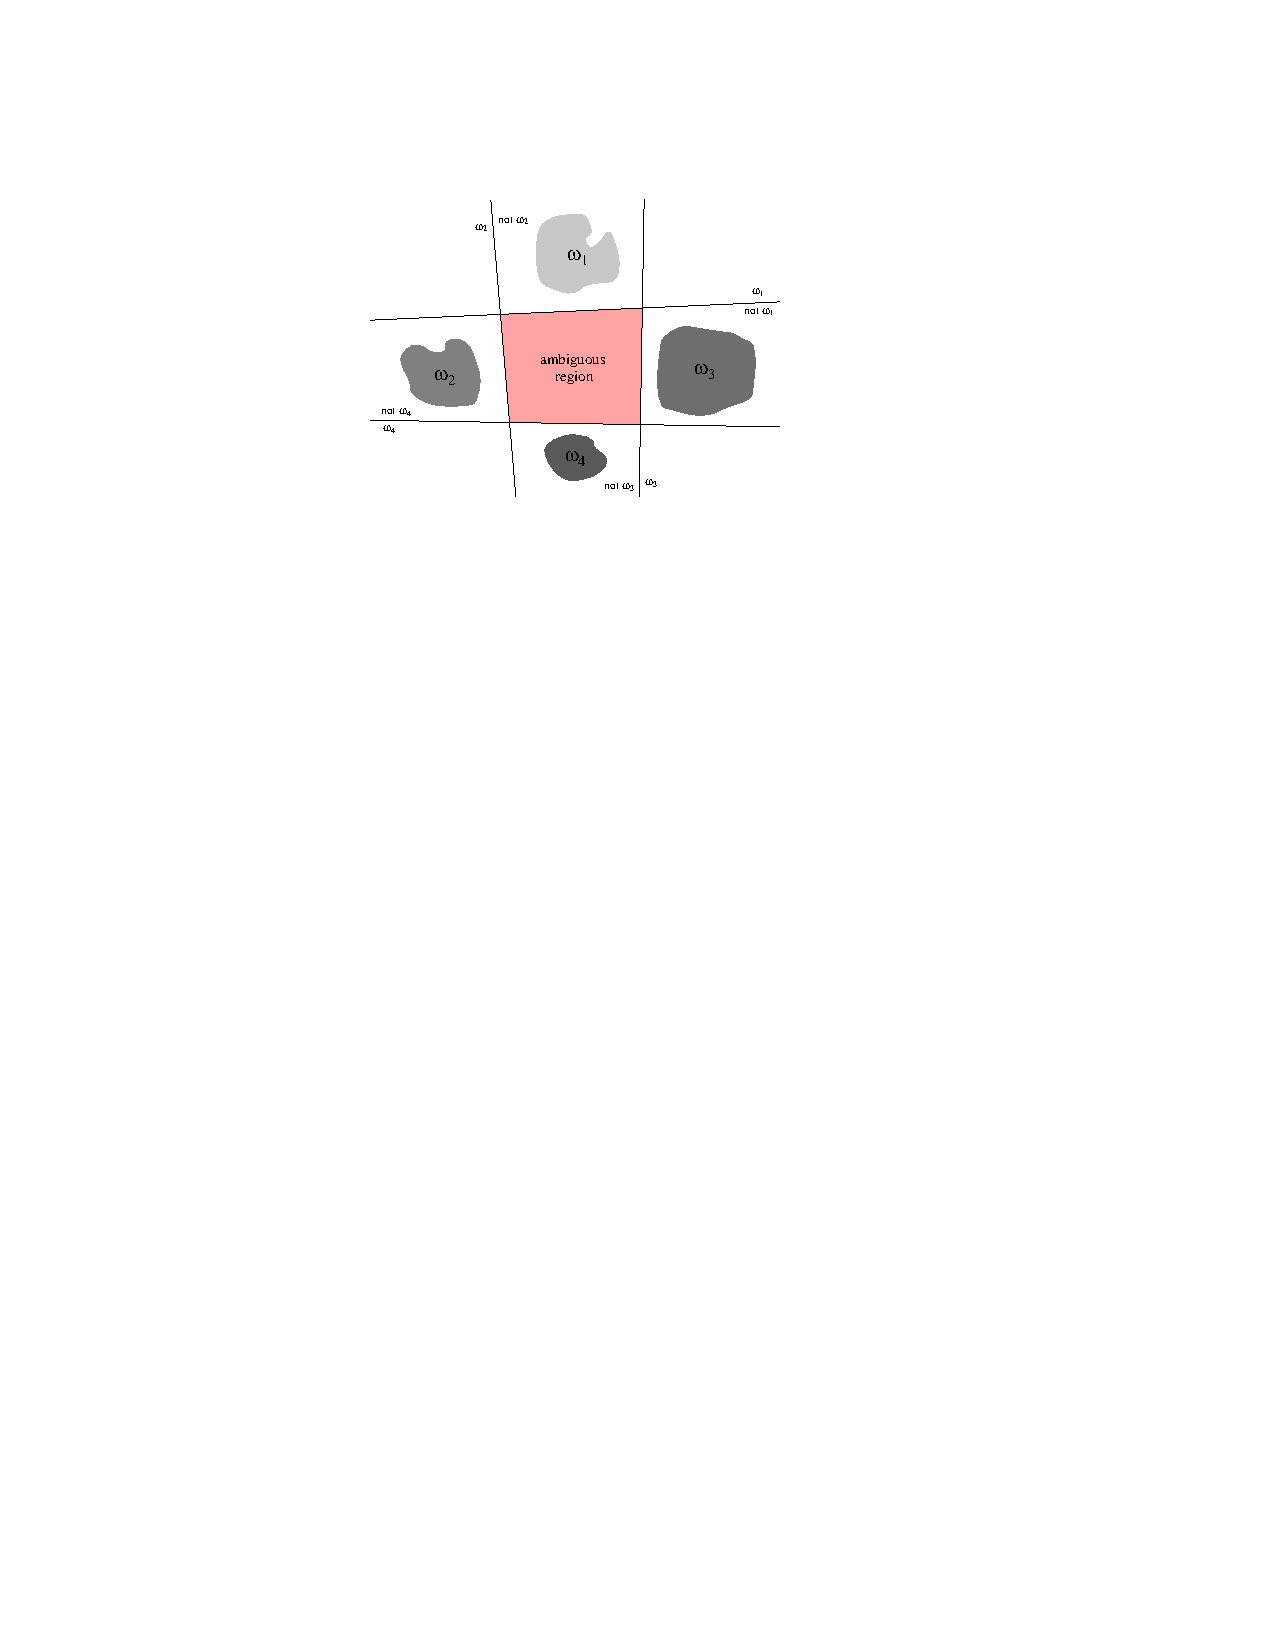
\includegraphics[scale=0.7]{ldf01}~~~~~~~
%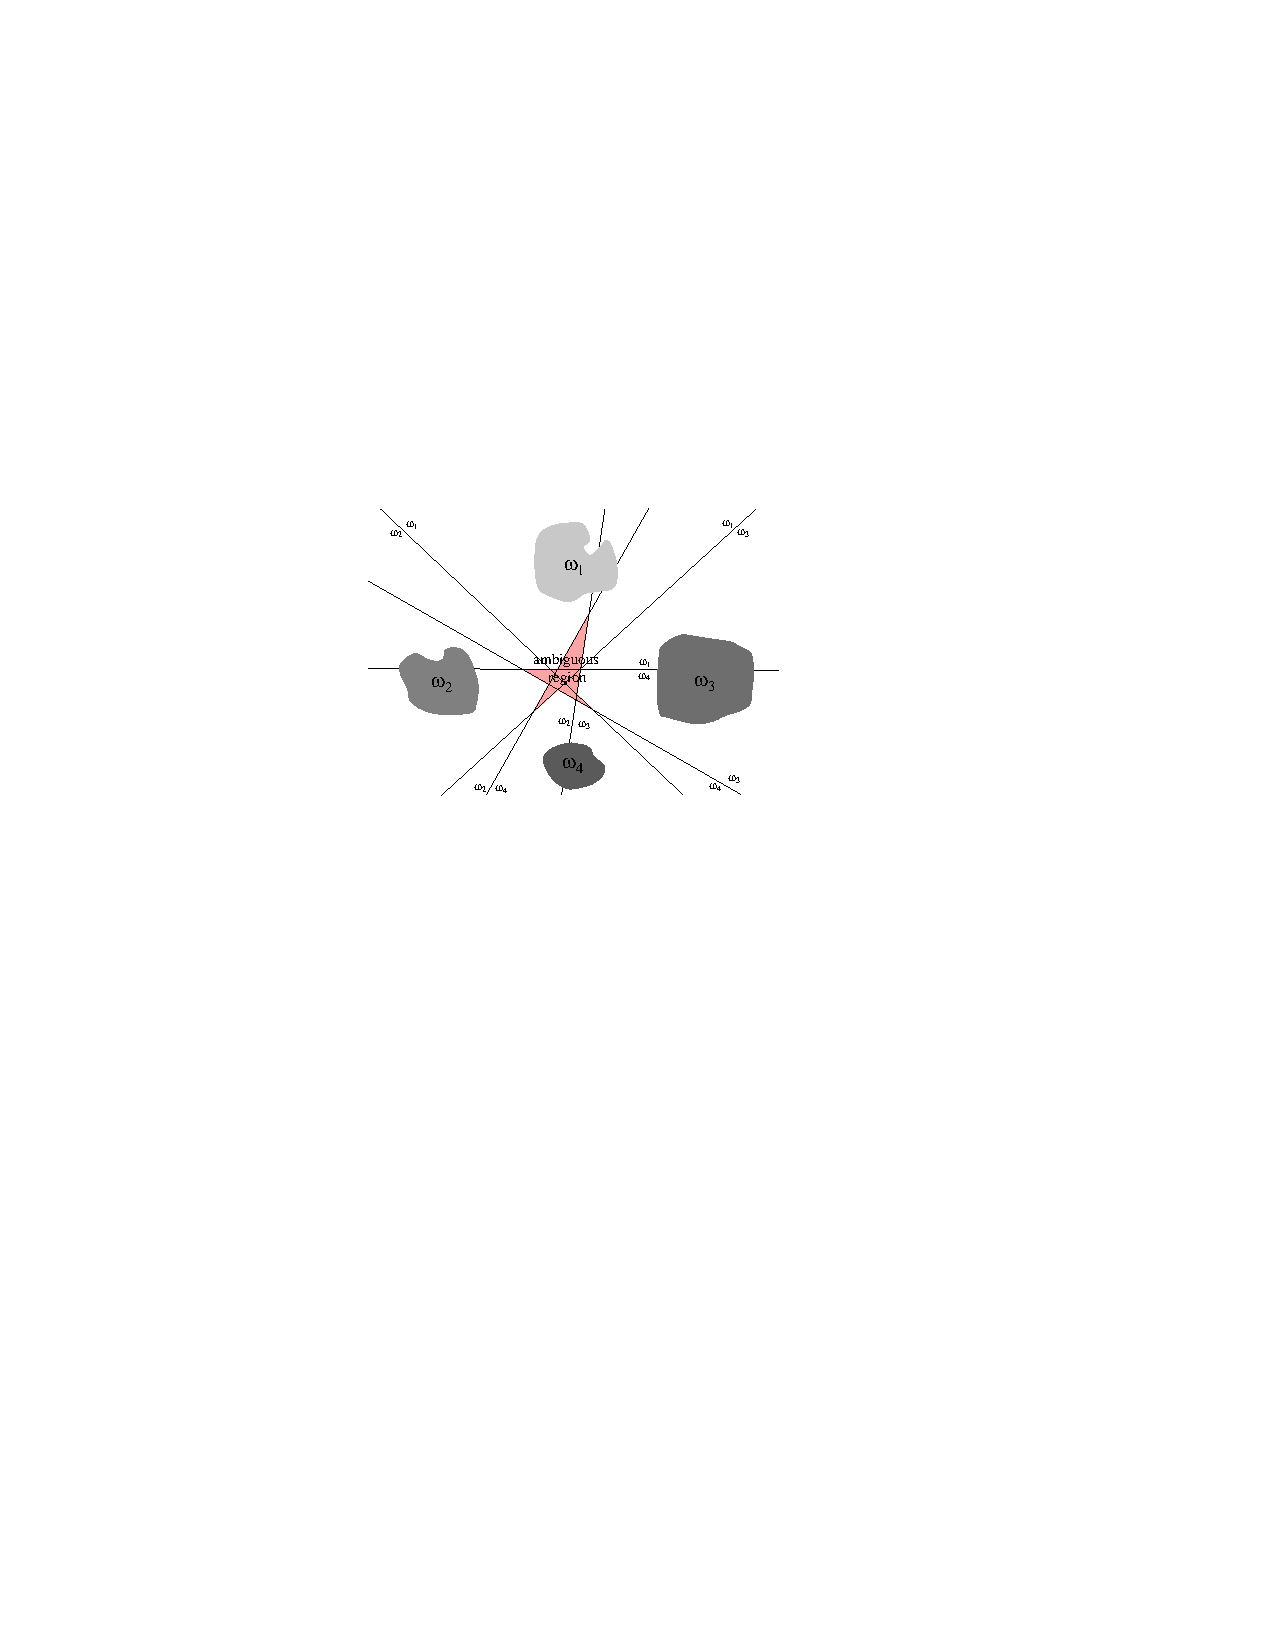
\includegraphics[scale=0.7]{ldf02}
%\caption{Linear decision boundaries fro a four-class problem devised as four two-class problems (left figure) and six pairwise problems (right figure). The pink regions have ambiguous category assignments.}
%\end{figure}
%\end{frame}

%\begin{frame}{The Multicategory Case}
%\begin{figure}
%\includegraphics[scale=0.8]{ldf03}
%\caption{Decision boundaries produced by a linear machine for a three-class problem and a five-class problem.}
%\end{figure}
%\end{frame}
\section{Generalized LDF}
\subsection{}
\begin{frame}{Generalized Linear Discriminant Functions}
\begin{itemize}
\item The linear discriminant function $g({\rm x})$ can be written as
\begin{equation}
g({\rm x}) = w_0+\sum_{i=1}^d w_ix_i
\end{equation}
%\begin{figure}
%
\includegraphics[scale=1]{ldf04}
%\end{figure}
where ${\rm w}=[w_1,\ldots,w_d]^T$
\item We can obtain the \textit{\color{mycolor2}quadratic discriminant function} by adding second-order terms as
\begin{equation}
g({\rm x}) = w_0+\sum_{i=1}^d w_ix_i+\sum_{i=1}^d\sum_{j=1}^dw_{ij}x_ix_j
\end{equation}
%\begin{figure}
%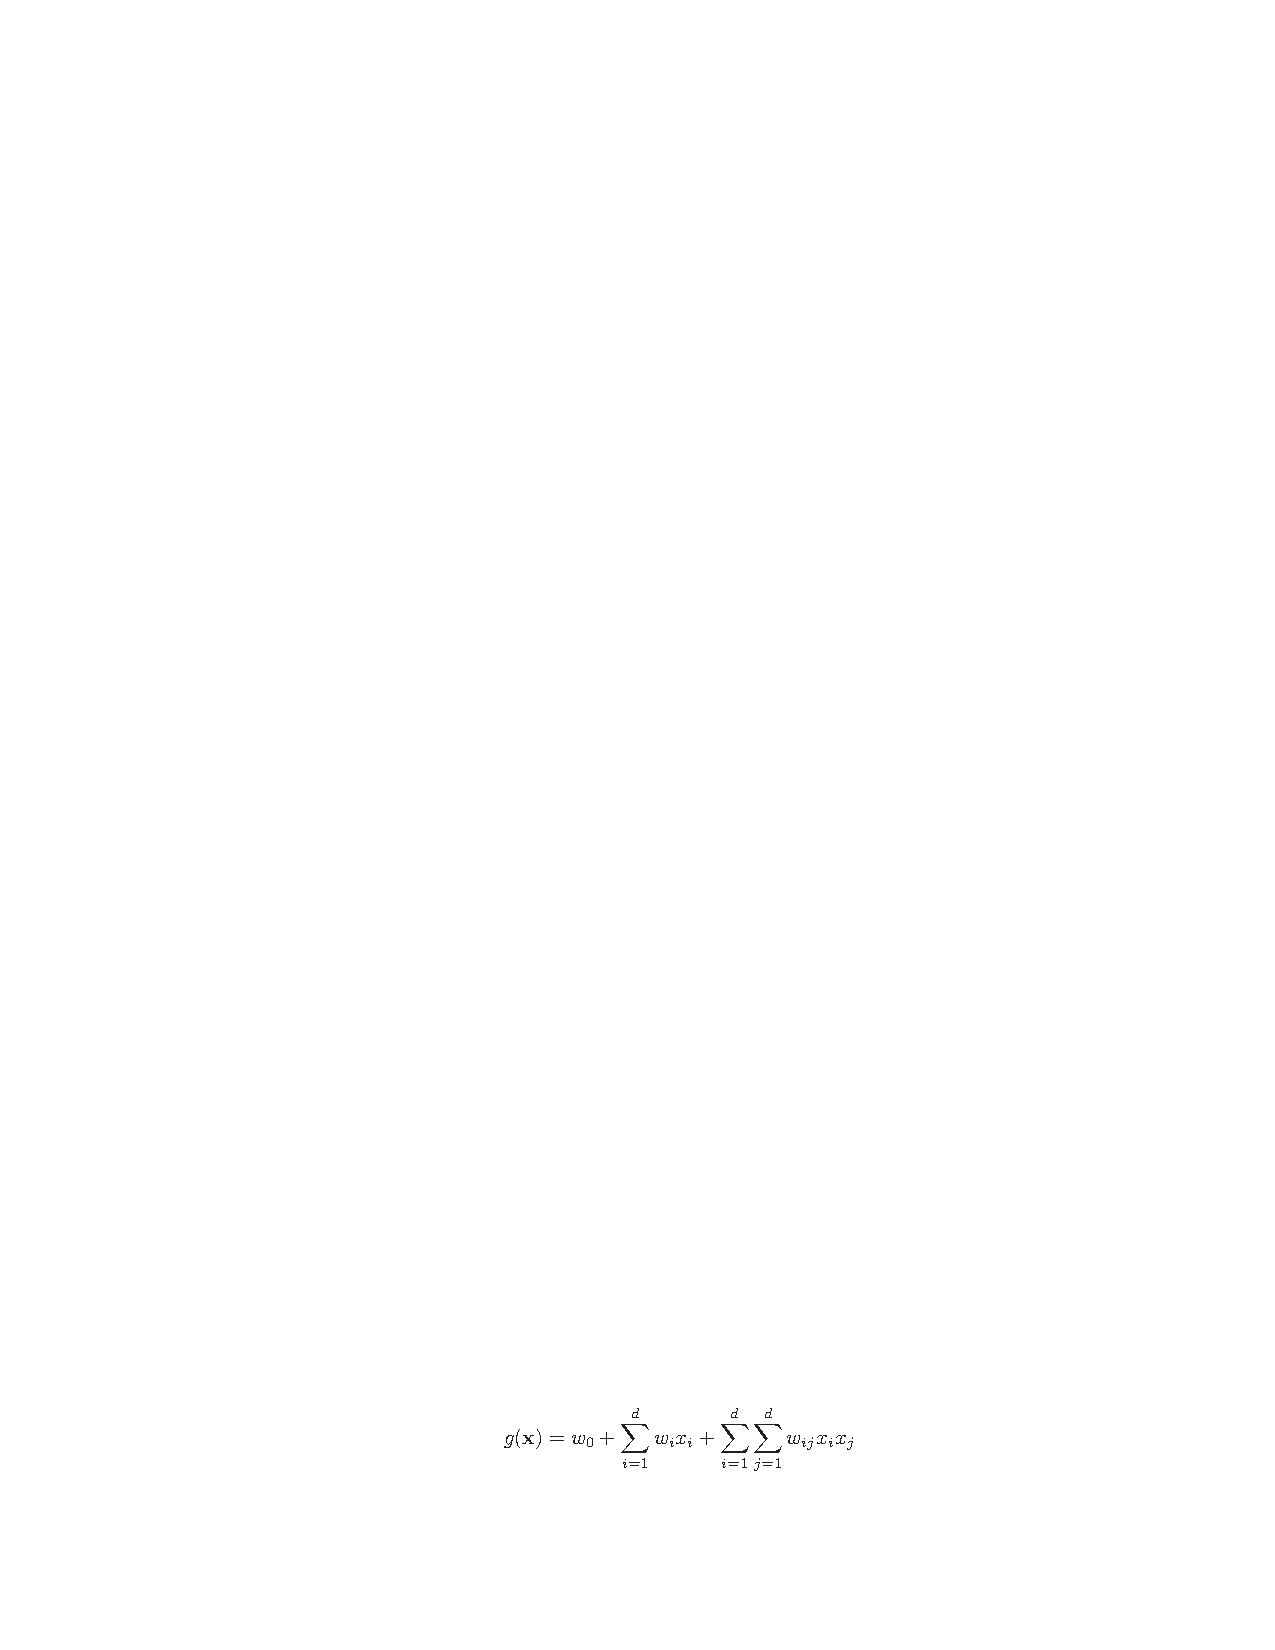
\includegraphics[scale=1]{ldf05}
%\end{figure}
Because $x_ix_j=x_jx_i$, we can assume that ${\rm w}_{ij}={\rm w}_{ji}$  with no loss in generality. Which result in more complicated decision boundaries.
({\color{mycolor2}hyperquadrics})
\end{itemize}
\end{frame}

\begin{frame}{Generalized Linear Discriminant Functions}
\begin{itemize}
\item The quadratic discriminant function has an additional $d(d+1)/2$ coefficients at its disposal with which to produce more complicated separating surfaces.
\item The separating surface defined by $g({\rm x})=0$ is a second-degree or hyperquadric surface.
\item If the symmetric matrix, ${\rm W} = [{\rm w}_{ij}]$, is nonsingular the linear term in $g({\rm x})$ can be eliminated by translating the axes. 
\item The basic character of the separating surface can be described in terms of scaled matrix
\begin{equation}
\bar{\rm W} = \frac{{\rm W}}{{{{\rm w}^T}{{\rm W}^{ - 1}}{\rm w} - 4{w_0}}} \nonumber
\end{equation}
where ${\rm w}=(w_1,\ldots,w_d)^T$ and ${\rm W}=[w_{ij}]$
\end{itemize}
\end{frame}

\begin{frame}{Generalized Linear Discriminant Functions}
The types of quadratic separating surfaces that arise in the general multivariate Gaussian case are as follows
\begin{itemize}
\item[1.] If $\bar{\rm W}$ is a positive multiple of the identity matrix, the separating surface is a \textit{\color{mycolor2}hypersphere} such that $\bar{\rm W}=kI$.
\item[2.] If $\bar{\rm W}$ is positive definite, the separating surfaces is a \textit{\color{mycolor3}hyperellipsoid} whose axes are in the direction of the eigenvectors of $\bar{\rm W}$.
\item[3.] If none of the above cases holds, that is, some of the eigenvalues of are positive and others are negative,
the surface is one of the varieties of types of \textit{\color{mycolor4}hyperhyperboloids}.
\end{itemize}
\end{frame}

\begin{frame}{Generalized Linear Discriminant Functions}
\begin{itemize}
\item By continuing to add terms such as $w_{ijk}x_ix_jx_k$, we can obtain the class of \textit{\color{mycolor2}polynomial discriminant functions}.
These can be thought of as truncated series expansions of some arbitrary $g ( {\rm x} )$, and this in turn suggest the
\textit{\color{mycolor2}generalized linear discriminant function}.
\begin{equation}
g({\rm x}) = \sum\limits_{i = 1}^{\hat d} {{a_i}{{\rm y}_i}({\rm x}) = {{\rm a}^T}{\rm y}} \nonumber
\end{equation}
where ${\rm a}$ is a $\hat{d}-$dimensional weight vector and $\hat{d}$ functions ${\rm y}_i({\rm x})$ are arbitrary functions of ${\rm x}$.
\item The physical interpretation is that the functions ${\rm y}_i({\rm x})$ map points ${\rm x}$ in $d$-dimensional space to point ${\rm y}$ in $\hat{d}$-dimensional space.
\end{itemize}
\end{frame}

\begin{frame}{Generalized Linear Discriminant Functions}
\begin{itemize}
\item Then, the discriminant $g({\rm x}) = {\rm a}^T {\rm y}$ separates points in the transformed space using a hyperplane passing through the origin.
\item This mapping to a higher dimensional space brings problems and additional requirements for computation and data.
\item However, certain assumptions can make the problem tractable.
\item Let the quadratic discriminant function be
\begin{equation}
g(x)=a_1+a_2{\rm x}+a_3{\rm x}^2 \nonumber
\end{equation}
\item So that the three-dimensional vector ${\rm y}$ is given by
\begin{equation}
{\rm y}=[1~~{\rm x}~~{\rm x}^2]^T \nonumber
\end{equation}
\item {\color{mycolor1}Kernel trick} implicitly maps their input into high-dimensional feature space.
\end{itemize}
\end{frame}

\begin{frame}{Generalized Linear Discriminant Functions}
\begin{figure}
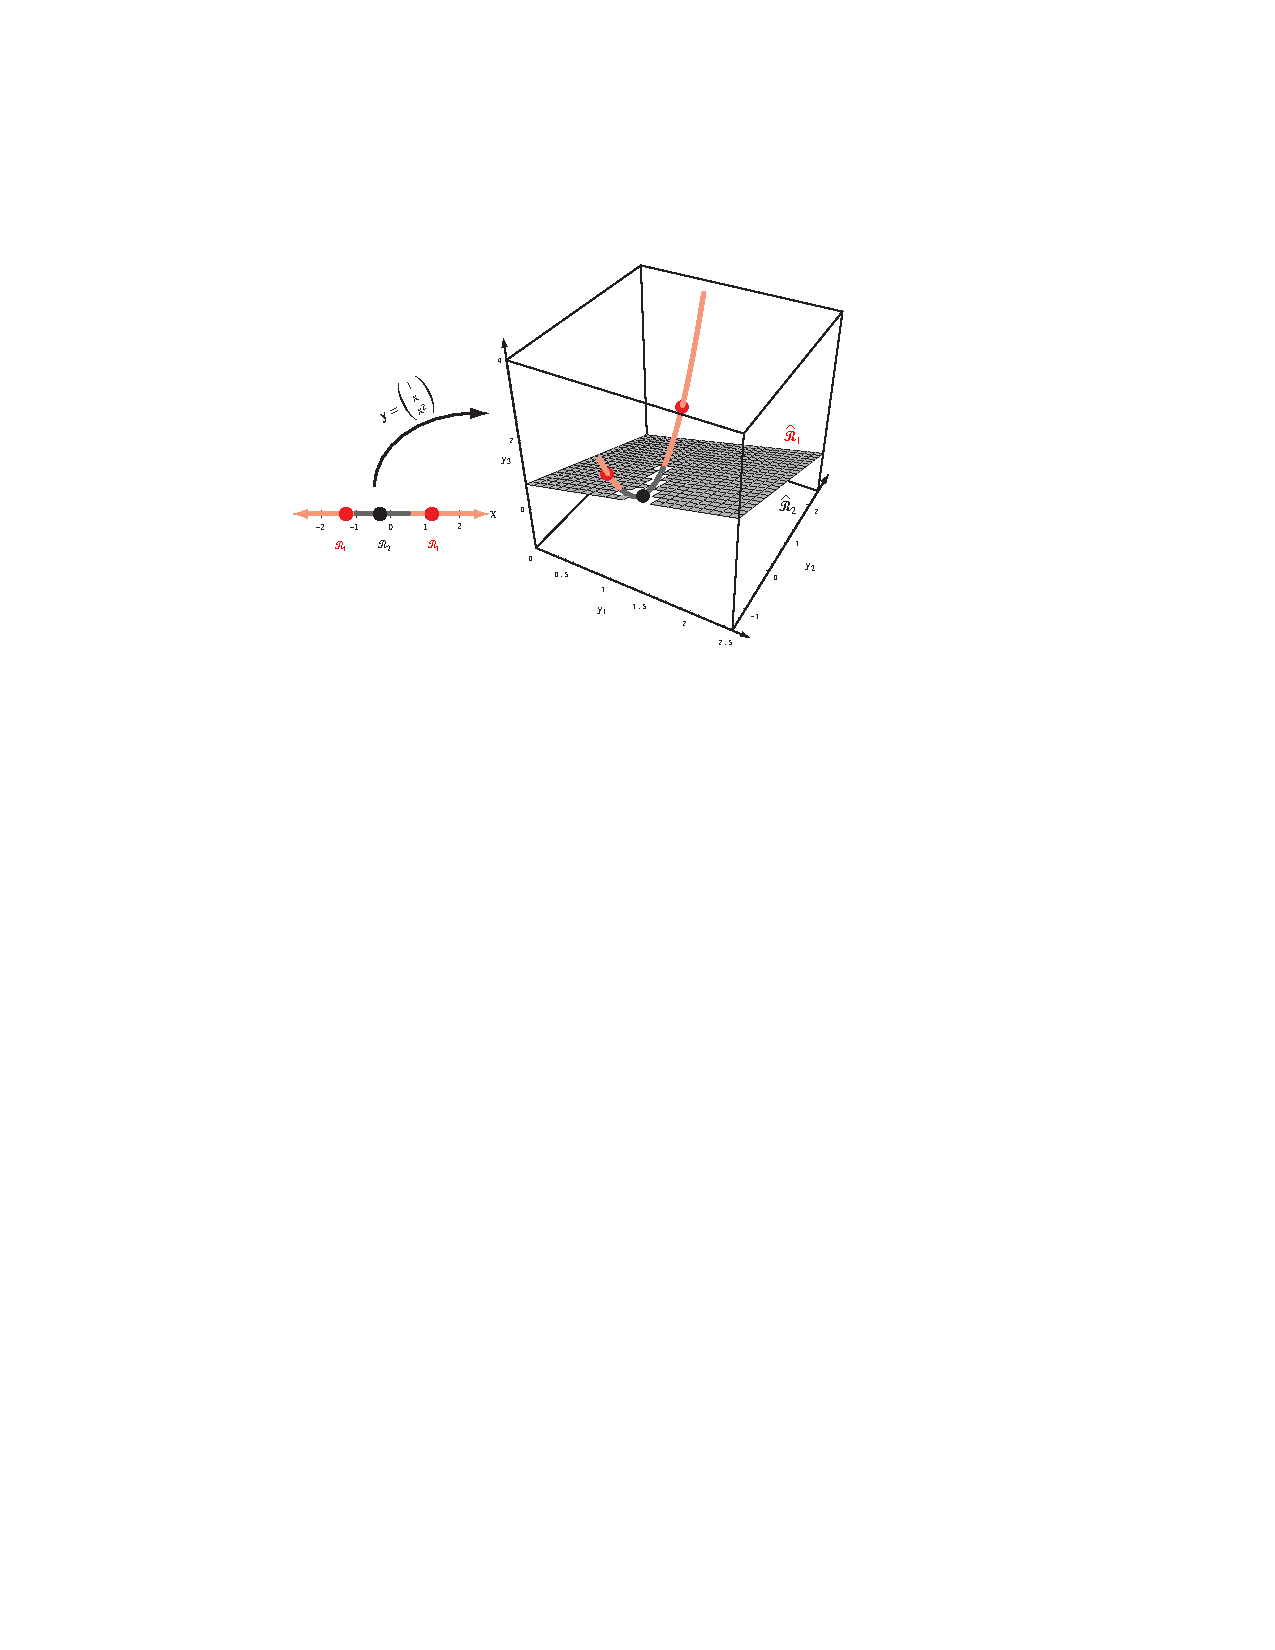
\includegraphics[scale=0.85]{ldf06}
\caption{The mapping ${\rm y} = (1~~ {\rm x}~~ {\rm x}^2 )^T$ takes a line and transforms it to a parabola
in three dimensions. A plane splits the resulting ${\rm y}$ space into regions corresponding
to two categories, and this in turn gives a non-simply connected decision region in the
one-dimensional ${\rm x}$ space.}
\end{figure}
\end{frame}

\begin{frame}{Generalized Linear Discriminant Functions}
\begin{figure}
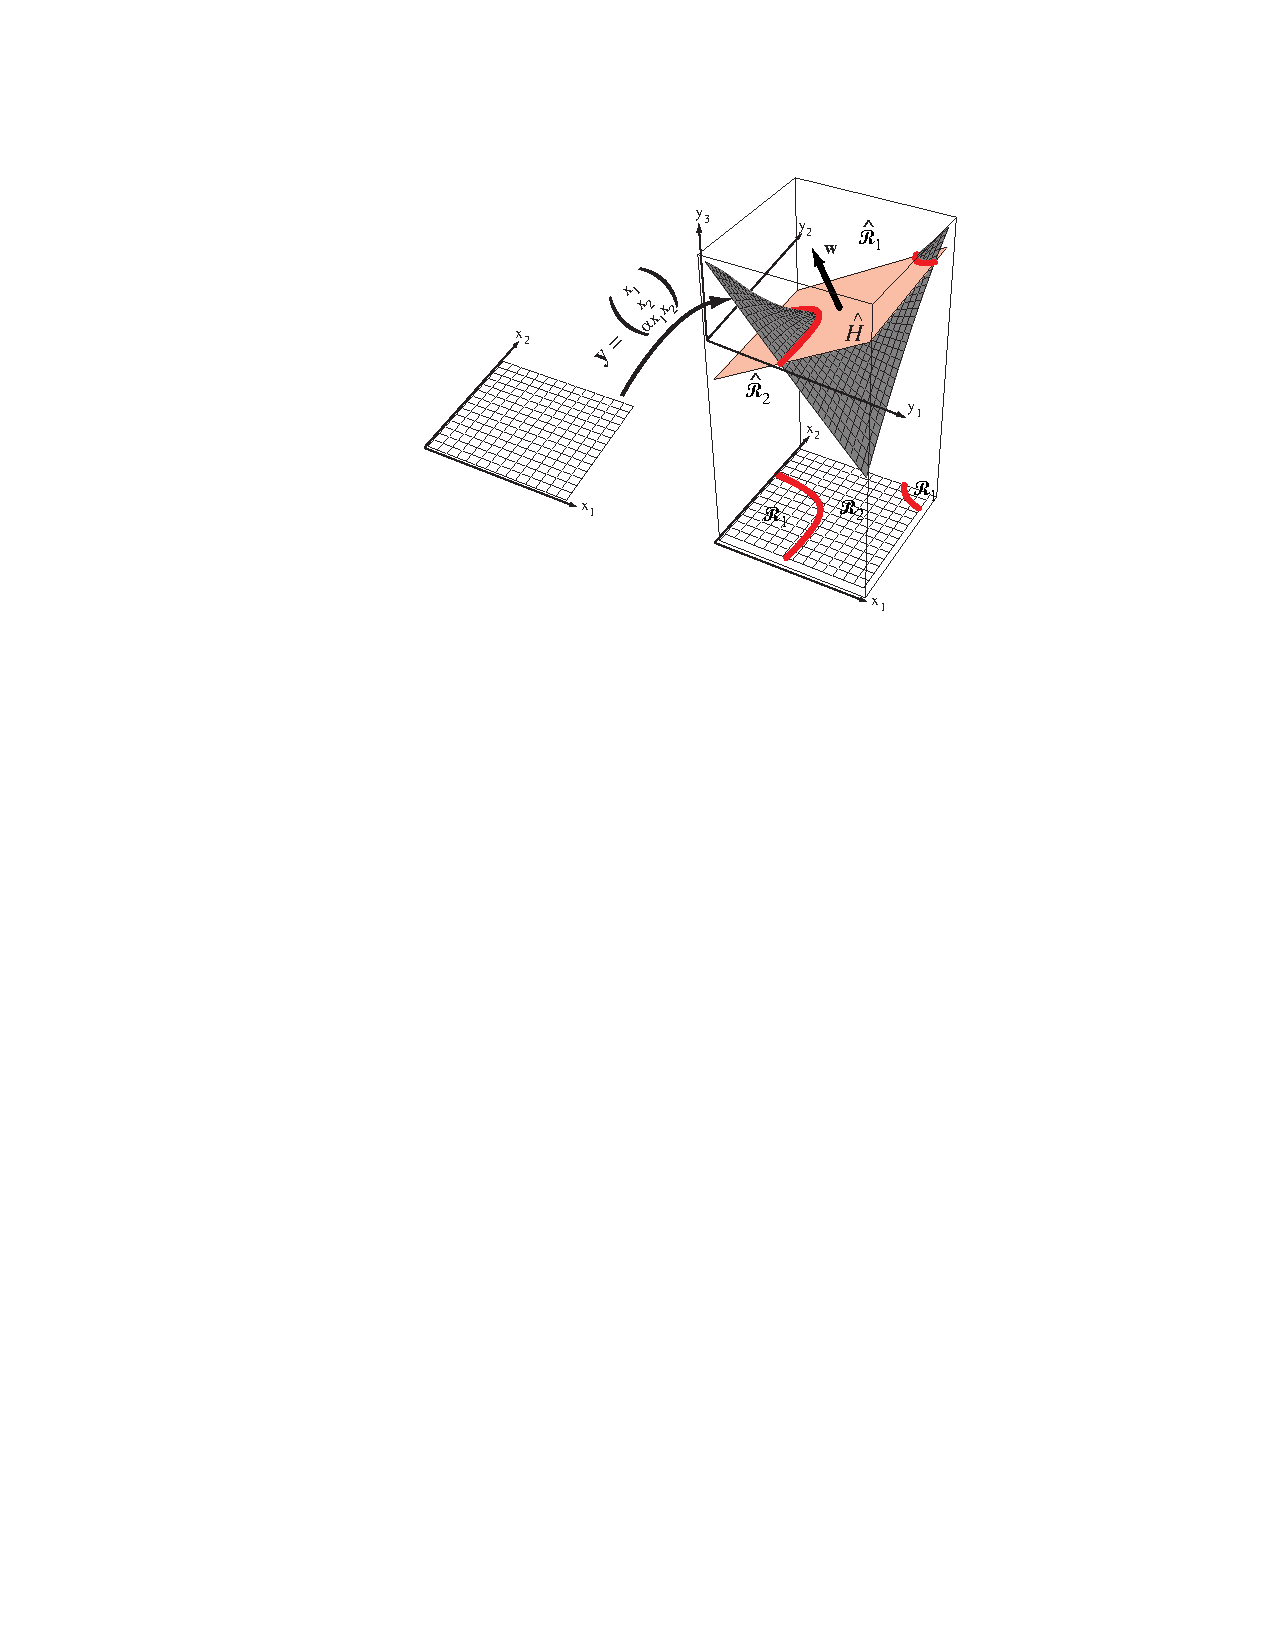
\includegraphics[scale=0.7]{ldf23}
\caption{The two-dimensional input space ${\rm x}$ is mapped through a polynomial
function $f$ to ${\rm y}$. Here the mapping is ${ y}_1 = {x}_1$ , ${y}_2 = {x}_2$ and ${y}_3\propto {x}_1 {x}_2$ . A linear
discriminant in this transformed space is a hyperplane, which cuts the surface. Points to the positive side of the hyperplane $\hat{H}$ correspond to category $\omega_1$ , and those beneath
it $\omega_2$ . Here, in terms of the ${\rm x}$ space, $\mathcal{R}_1$ is a not simply connected.}
\end{figure}
\end{frame}

%\begin{frame}{Topics}
%\begin{itemize}
%\item Linear Discriminant Functions and Decision Surfaces
%\item Generalized Linear Discriminant Functions
%\item The two-category linearly separable case
%\item Perceptron Criterion
%\item Criterion Function
%\item Minimum Squared Error Procedures
%\item The Ho-Kashyap Procedures
%\end{itemize}
%\end{frame}
%
%
%\begin{frame}{Introduction}
%\begin{itemize}
%\item Linear Discriminant Functions and Decisions   Surfaces
%\item Generalized Linear Discriminant Functions
%\end{itemize}
%\end{frame}
%

\section{Support Vector Machine}
\subsection{}
\begin{frame}{}
\begin{variableblock}{\centering \Large \textbf{\vspace{4pt}\newline Support Vector Machine\vspace{4pt}}}{bg=slidecolor,fg=white}{bg=slidecolor,fg=white}
\end{variableblock}
\end{frame}

\begin{frame}{Introduction}
\begin{itemize}
\item Support vector machines (SVMs) are a linear machines initially developed for two class problems.
\item SVMs are a set of supervised learning methods used for 
\begin{itemize}
\item classification, 
\item regression and 
\item outliers detection.
\end{itemize}
\item The advantages of support vector machines are:
\begin{itemize}
\item Effective in high dimensional spaces.
\item Still effective in cases where number of dimensions is greater than the number of samples.
\item Uses a subset of training points in the decision function (called {\color{mycolor2}support vectors}), so it is also {\color{mycolor1}memory efficient}.
\item Versatile: different SVM kernels can be specified for the decision function. Common kernels are provided, but it is also possible to specify custom kernels.
\end{itemize}
\end{itemize}
\end{frame}


\begin{frame}{Introduction}
\begin{itemize}
\item The disadvantages of support vector machines include:
\begin{itemize}
\item If the number of features is much greater than the number of samples then choosing regularization to avoiding over-fitting is crucial. 
\item SVMs do not directly provide probability estimates, these are calculated using an expensive five-fold cross-validation.
\end{itemize}
\item In addition to performing linear classification, SVMs can efficiently perform a non-linear classification using what is called {\color{mycolor1}Kernel trick}.
\item Kernel trick implicitly maps their input into high-dimensional feature space.
\end{itemize}
\end{frame}

\begin{frame}{Linear decision boundary}
\begin{itemize}
\item Binary classification can be viewed as the task of separating classes in feature space using decision boundary:
\begin{figure}
\includegraphics[scale=0.5]{Figures/data4.pdf}
\end{figure}
\[f({\rm x})=\text{sign}({\rm w}^T{\rm x}+b)\]
\end{itemize}
\end{frame}

\begin{frame}{What is a good Decision Boundary?}
\begin{itemize}
\item Which of the linear separators is optimal?
\item Consider a two-class, linearly
separable classification problem
\item  Many decision boundaries are possible.
\item  The perceptron algorithm can be
used to find such a boundary.
\item Are all decision boundaries equally
good?
\end{itemize}
\begin{figure}
\includegraphics[scale=0.45]{Figures/data2.pdf}
\end{figure}
\end{frame}

\begin{frame}{Linear SVM: Objective}
\begin{itemize}
\item Let us training data set, $\mathcal{D}$, a set of $n$ points.
\[\mathcal{D}=\{({\rm x}_i,y_i)~~|~~{\rm x}_i\in \Re ^d, y_i\in \{-1,1\}\}^n_{i=1}\]
${\rm x}_i~~\rightarrow$~~$d$-dimensional real vector
\item {\rm Objective}: find maximum-margin hyperplane 
\[{\rm w}^T{\rm x}+b=0\]
where ${\rm w}$ is the normal vector to the hyperplane and $b$ is the bias/intercept.
\begin{figure}
\includegraphics[scale=0.3]{data0}~~~
\includegraphics[scale=0.3]{data1}
\end{figure}
\end{itemize}
\end{frame}


\begin{frame}{Linear SVM: pictorial representation}
\begin{figure}
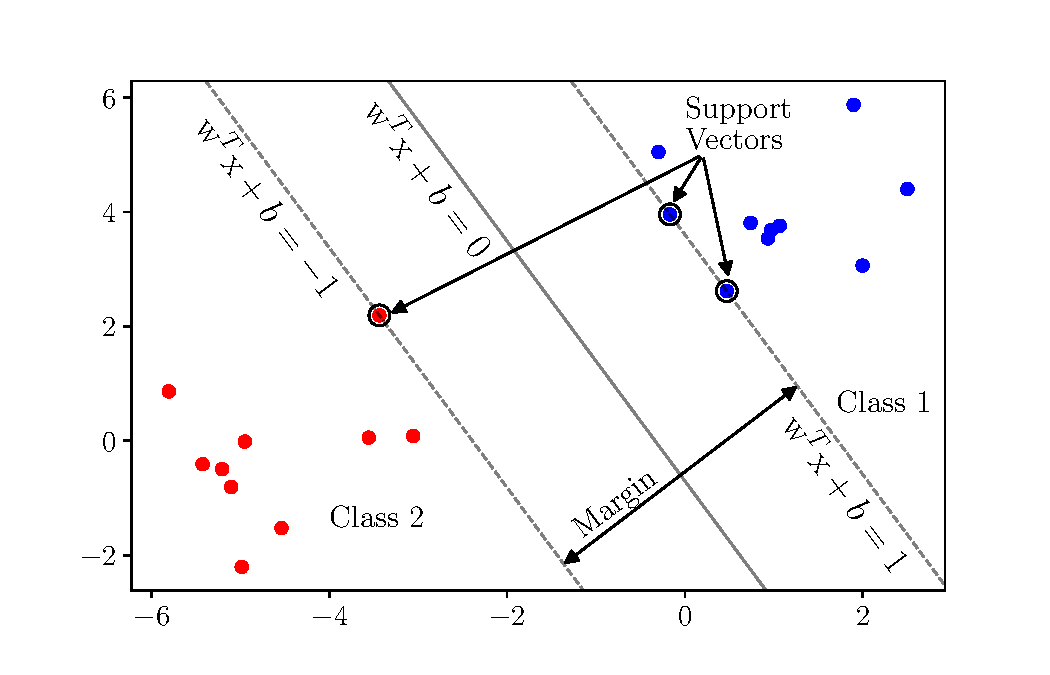
\includegraphics[scale=0.55]{Figures/data5}
\end{figure}
\end{frame}

\begin{frame}{Preliminary concepts}
\begin{itemize}
\item Let ${\rm x}_n$ be the nearest data point to the plane ${\rm w}^T{\rm x}+b=0$. 
\item How far is it?
\item Normalize ${\rm w}$ and $b$ such that:
\[|{\rm w}^T{\rm x}_n+b|=1\]
\end{itemize}
\begin{columns}
\begin{column}{6cm}
\vspace{-12pt}
\begin{itemize}
\item Now, we need to compute the distance between ${\rm x}_n$ and the plane ${\rm w}^T{\rm x}+b=0$, where $|{\rm w}^{T}{\rm x}_n+b|=1$.
\item The vector ${\rm w}$ is $\perp$ to the plane in the $\mathcal{X}$ space:
\item Take ${\rm x}'$ and ${\rm x}''$ on the plane
\[{\rm w}^T{\rm x}'+b=0~~\text{and}~~{\rm w}^T{\rm x}''+b=0\]
\end{itemize}
\end{column}
\begin{column}{4.5cm}
\begin{figure}
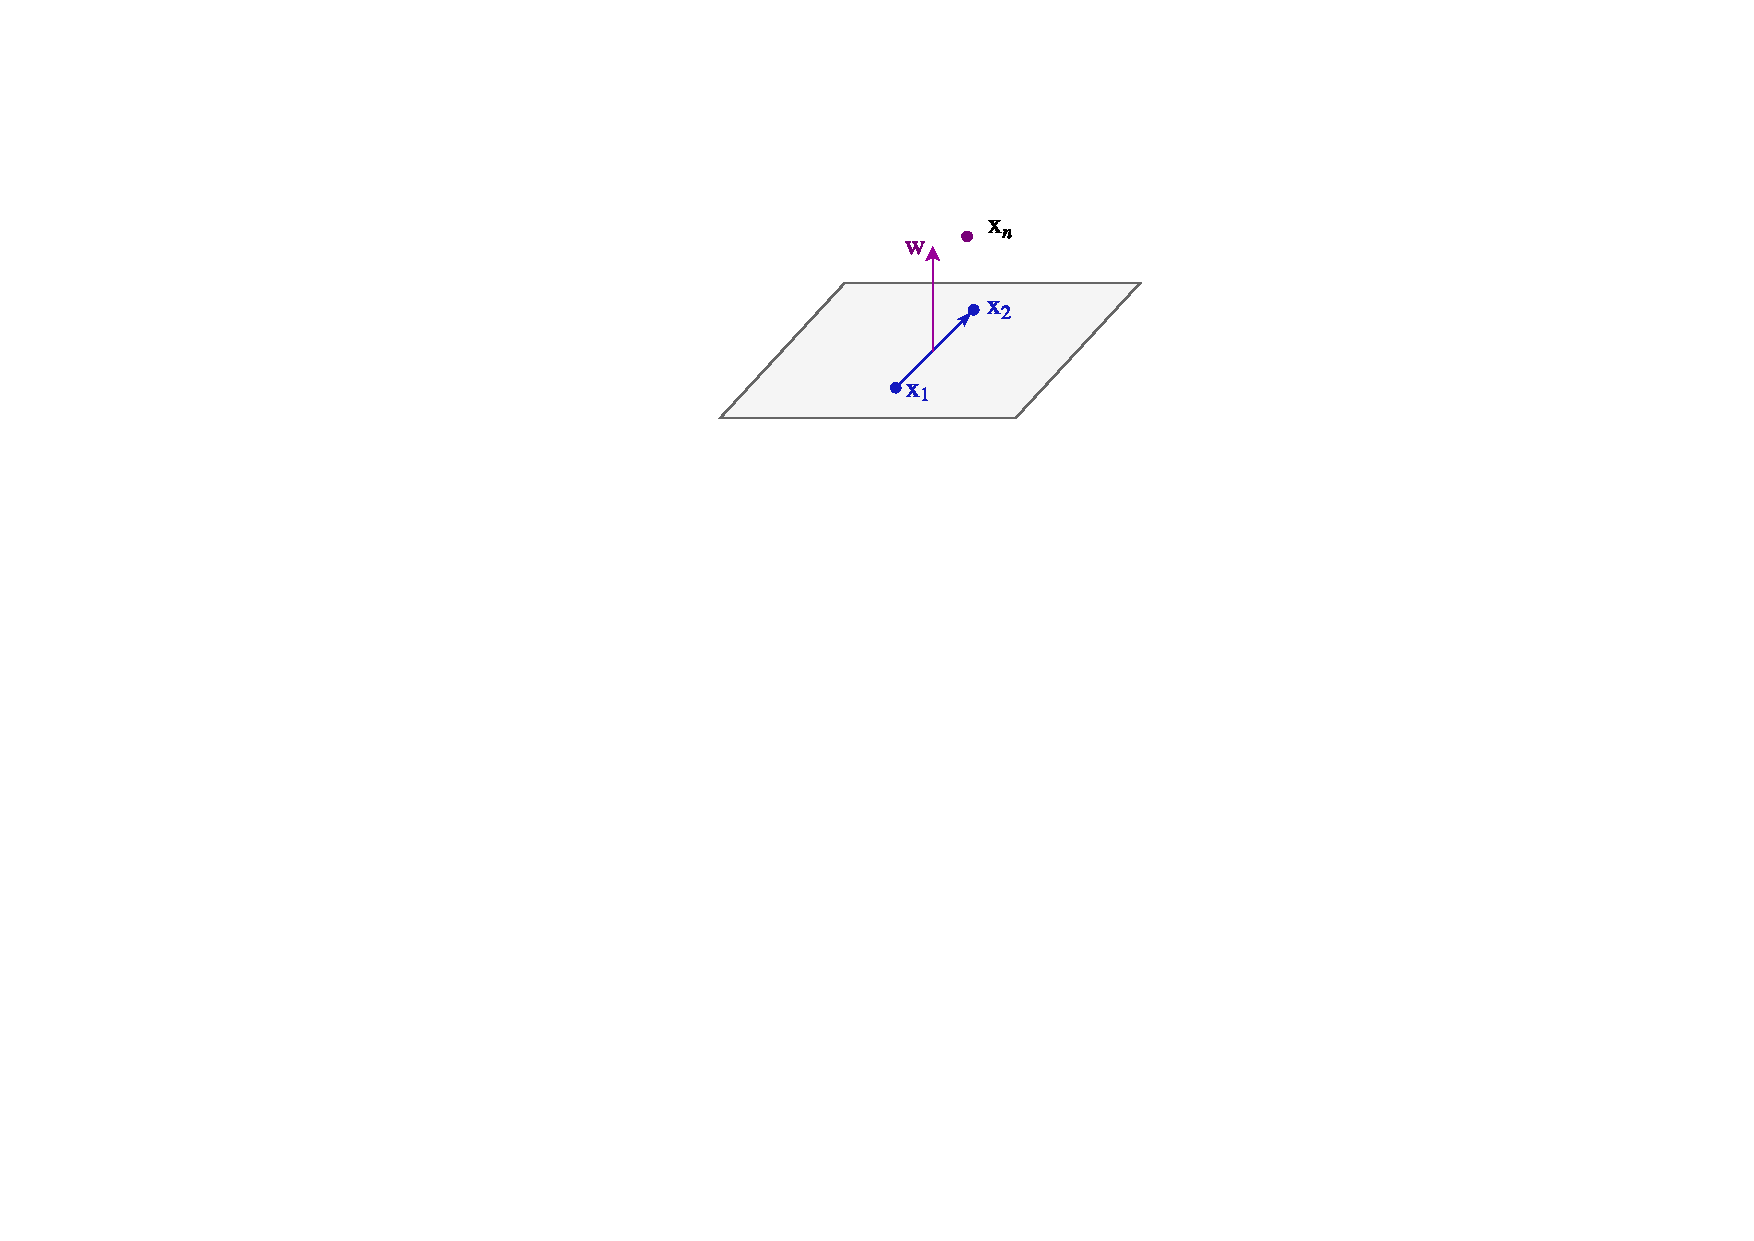
\includegraphics[scale=0.15]{SVM01.png}
\end{figure}
\[\Rightarrow~~ {\rm w}^T({\rm x}'-{\rm x}'')=0\]
\end{column}
\end{columns}
\end{frame}

\begin{frame}{Preliminary concepts}
The distance between ${\rm x}_n$ and the plane:
\begin{columns}
\begin{column}{4cm}
\begin{figure}
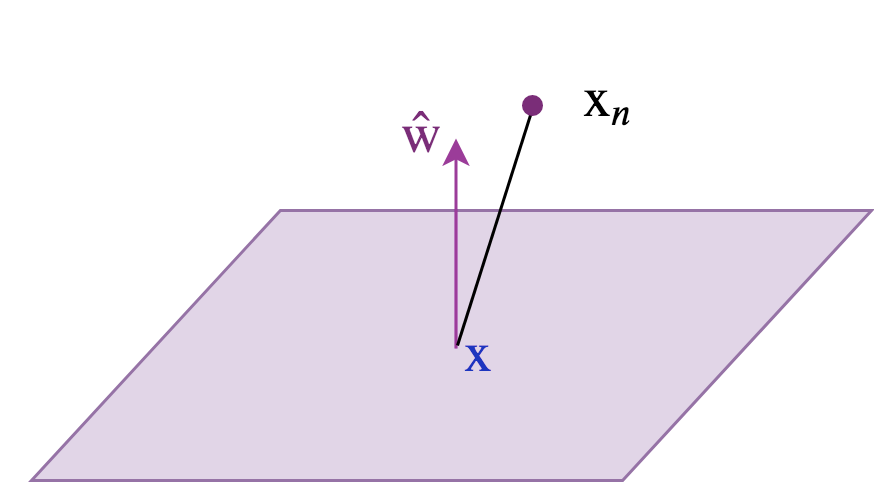
\includegraphics[scale=0.6]{Figures/SVM02.png}
\end{figure}
\end{column}
\begin{column}{6cm}
\begin{itemize}
\item Take any point ${\rm x}$ on the plane
\item Projection of ${\rm x}_n-{\rm x}$ on $\hat{\rm w}$
\[\hat{\rm w}=\frac{\rm w}{||\rm w||}\]
\[\Rightarrow ~~\text{distance}=|\hat{\rm w}^T({\rm x}_n-{\rm x})|\]
%
%${\rm w}^T{\rm x}+b=0$, where $|{\rm w}^{T}{\rm x}_n+b|=1$.
%\item The vector ${\rm w}$ is $\perp$ to the plane in the $\mathcal{X}$ space:
%\item Take ${\rm x}'$ and ${\rm x}''$ on the plane
%\[{\rm w}^T{\rm x}'+b=0~~\text{and}~~{\rm w}^T{\rm x}''+b=0\]
%\[\Rightarrow~~ {\rm w}^T({\rm x}'-{\rm x}'')=0\]
\end{itemize}

\end{column}
\end{columns}
\[\text{distance} = \frac{1}{||{\rm w}||}|{\rm w}^T{\rm x}_n-{\rm w}^T{\rm x}|= \frac{1}{||{\rm w}||}|{\rm w}^T{\rm x}_n+b-{\rm w}^T{\rm x}-b|=\frac{1}{||{\rm w}||}\]
\end{frame}


\begin{frame}{Problem formulation}
\begin{columns}
\begin{column}{6cm}
\begin{figure}
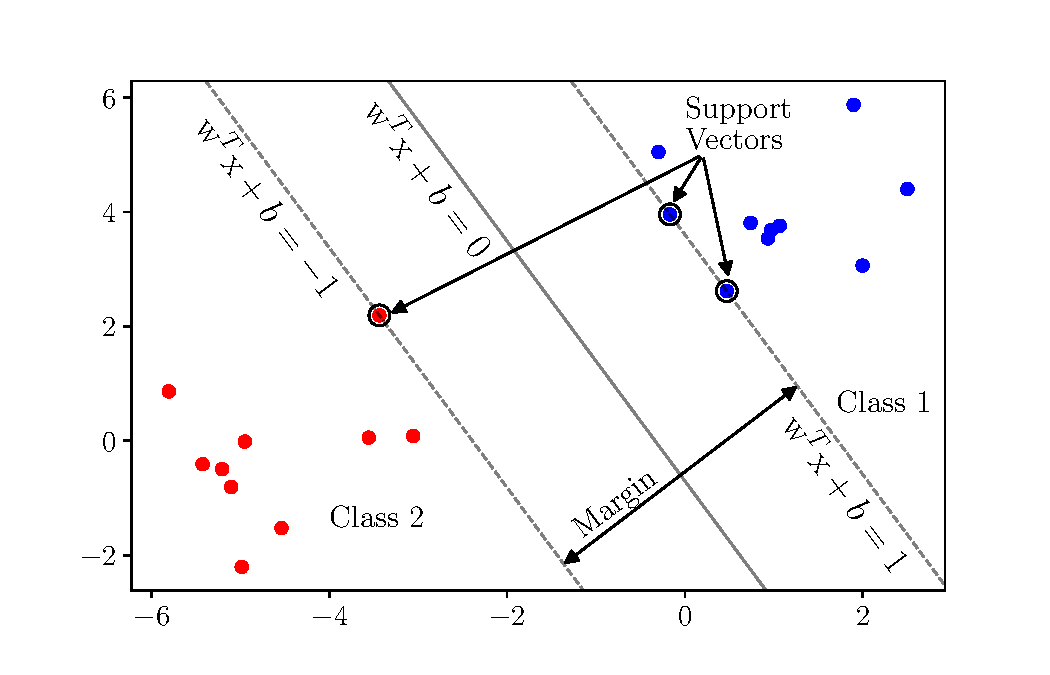
\includegraphics[scale=0.43]{Figures/data5}
\end{figure}
\end{column}
\begin{column}{5cm}

\begin{itemize}
\item Two hyperplanes
\begin{align*}
{\rm w}^T{\rm x}+b=&1\\
{\rm w}^T{\rm x}+b=&-1
\end{align*}
\item So the distance between the hyperplane is
\[\frac{b+1}{||{\rm w}||}-\frac{b-1}{||{\rm w}||}=\frac{2}{||{\rm w}||}\]
(need to be maximize)
\item Therefore, $||{\rm w}||$ need to be minimize.
\end{itemize}
\end{column}
\end{columns}
\end{frame}

\begin{frame}{Problem formulation}
\begin{itemize}
\item Therefore, we need to minimize $||{\rm w}||$ to maximize the margin.
\item We also have to restrict data points from falling into the margin, so add the following constraints:
\begin{itemize}
\item ${\rm w}^T{\rm x}_i+b\geq 1$ for ${x}_i$ of the 1st class.
\item ${\rm w}^T{\rm x}_i+b\leq -1$ for ${x}_i$ of the 2nd class.
\end{itemize}
\item This can be written as
\[y_i({\rm w}^T{\rm x}_i+b)\geq 1~~~\text{for}~~~i=1,2,\ldots,n\]
\item Combining the above two
\begin{align*}
&\mathop{\sf Minimize}\limits_{{\rm w},b}~~||{\rm w}||\\
&\text{subject to}~~y_i( {{{\rm w}^T}{{\rm x}_i} + b} ) \geq 1~~~\text{for}~~~i=1,2,\ldots,n
\end{align*}
\end{itemize}
\end{frame}

\begin{frame}{Problem formulation}
%\begin{align*}
%&\text{Maximize}~~\frac{1}{{\left\| {\rm w} \right\|}}\\
%&\text{subject to}\mathop {\min }\limits_{n = 1,2, \ldots N} \left| {{{\rm w}^T}{{\rm x}_n} + b} \right| = 1~~~~~~~~~~~~~~~~~~~~~~~~
%\end{align*}
%Notice: $\left| {{{\rm w}^T}{{\rm x}_n} + b} \right|=y_n( {{{\rm w}^T}{{\rm x}_n} + b} )$
\begin{itemize}

\item Problem is difficult to solve because it depends on $||{\rm w}||$, the norm of ${\rm w}$, which involves a square root.
\item Substitute $||{\rm w}||$ with $\frac{1}{2}||{\rm w}||^2$ (just for mathematical convenience)
\item Then problem is formulated as

\begin{align*}
&\mathop{\sf Minimize}\limits_{{\rm w},b}~~\frac{1}{2}||{\rm w}||^2\\
&\text{subject to}~~y_i( {{{\rm w}^T}{{\rm x}_i} + b} ) \geq 1~~~~\text{for}~~~i=1,2,\ldots,n
\end{align*}
\item The above problem is {\color{mycolor1}constraint optimization problem}.
\end{itemize}
\end{frame}


\begin{frame}{Problem solution: Lagrange formulation}
\begin{itemize}
\item There is no direct solution of the above constraint problem.
\item To obtain the dual, take positive Lagrange multiplier $\alpha_i$ multiplied by each constraint and subtract from the objective function.
\[{\sf Minimize}~~~\mathcal{L}({\rm w},b,\alpha)=\frac{1}{2}{\rm w}^T{\rm w} -\sum_{i=1}^{n} \alpha_i (y_i({\rm w}^T{\rm x}_i+b)-1)\]
w.r.t. ${\rm w}$ and $b$ and maximize w.r.t. each $\alpha_{i}\geq 0$
\item We can find the constraint as
\[\begin{gathered}
  {\nabla _{\rm w}}\mathcal{L} = {\rm w} - \sum\limits_{i = 1}^n {{\alpha _i}{y_i}{{\rm x}_i} = 0}  \hfill \\
  \frac{{\partial \mathcal{L}}}{{\partial b}} =  - \sum\limits_{i = 1}^n {{\alpha _i}{y_i} = 0}  \hfill \\ 
\end{gathered} \]
\end{itemize}
\end{frame}

%\begin{frame}{Constrained optimization}
%\begin{figure}
%\includegraphics[width=\textwidth]{SVM03}
%\end{figure}
%\end{frame}

%\begin{frame}{We saw this before}
%\begin{figure}
%\includegraphics[width=\textwidth]{SVM04}
%\end{figure}
%\end{frame}

%\begin{frame}{Lagrange formulation}
%\begin{figure}
%\includegraphics[width=\textwidth]{SVM05}
%\end{figure}
%\end{frame}

\begin{frame}{Problem solution: Lagrange formulation}
\begin{itemize}
\item We obtained
\[ {\rm w} = \sum\limits_{i = 1}^n {{\alpha _i}{y_i}{{\rm x}_i}}    ~~~~~~~ \text{and} ~~~~~~~    \sum\limits_{i = 1}^n {{\alpha _i}{y_i} = 0} \]
\item Substitute in Lagrangian optimization problem,
\[\mathcal{L}({\rm w},b,\alpha ) = \frac{1}{2}{{\rm w}^T}{\rm w} - \sum\limits_{i = 1}^n {{\alpha _i}({y_i}({{\rm w}^T}{{\rm x}_i} + b) - 1)} \]
 we get
 \[\mathcal{L}(\alpha ) = \sum_{n=1}^{n}\alpha_n -\frac{1}{2}\sum_{i=1}^{n} \sum\limits_{j= 1}^n y_iy_j\alpha_i\alpha_j {\rm x}_i^T{\rm x}_j\]
 Maximize w.r.t. to $\alpha$ subject to $\alpha_i\geq 0$ for $i=1,\ldots,n$ and $\sum_{i=1}^n\alpha_iy_i =0$
\end{itemize}
\end{frame}

\begin{frame}{The solution - quadratic programming}
\[\begin{gathered}
  \mathop {\min }\limits_\alpha ~~~ \frac{1}{2}{\alpha ^T}\left[ {\begin{array}{*{20}{c}}
  {{y_1}{y_1}x_1^T{x_1}}&{{y_1}{y_2}x_1^T{x_2}}&{\cdots}&{{y_1}{y_n}x_1^T{x_n}} \\ 
  {{y_2}{y_1}x_2^T{x_1}}&{{y_2}{y_2}x_2^T{x_2}}&{\cdots}&{{y_2}{y_n}x_2^T{x_n}} \\ 
  {\vdots}&{\vdots}&{\ddots}&{\vdots} \\ 
  {{y_n}{y_1}x_n^T{x_1}}&{{y_n}{y_2}x_n^T{x_2}}&{\cdots}&{{y_n}{y_n}x_n^T{x_n}} 
\end{array}} \right]\alpha  + \left( { - {1^T}} \right)\alpha  \hfill \\\\
  \text{subject to   }{y^T}\alpha  = 0\text{   and   }0 \leqslant \alpha  \leqslant \infty  \hfill \\ 
\end{gathered} \]
\end{frame}

%\begin{frame}{Substituting...}
%\begin{figure}
%\includegraphics[width=\textwidth]{SVM06}
%\end{figure}
%\end{frame}

\begin{frame}{Example: Linear (trivial problem)}
Suppose we are given the following positively labeled data points in $\Re^2$:
\[\left\{ {\left( {\begin{array}{*{20}{c}}
  3 \\ 
  1 
\end{array}} \right),\left( {\begin{array}{*{20}{c}}
  3 \\ 
  { - 1} 
\end{array}} \right),\left( {\begin{array}{*{20}{c}}
  6 \\ 
  1 
\end{array}} \right),\left( {\begin{array}{*{20}{c}}
  6 \\ 
  { - 1} 
\end{array}} \right)} \right\}\]
and the following negatively labeled data points in $\Re^2$
\[\left\{ {\left( {\begin{array}{*{20}{c}}
  1 \\ 
  0 
\end{array}} \right),\left( {\begin{array}{*{20}{c}}
  0 \\ 
  { 1} 
\end{array}} \right),\left( {\begin{array}{*{20}{c}}
  0 \\ 
  -1 
\end{array}} \right),\left( {\begin{array}{*{20}{c}}
  -1 \\ 
  { 0} 
\end{array}} \right)} \right\}\]
\begin{figure}
\includegraphics[scale=0.35]{data6.pdf}
\end{figure}
\end{frame}

%\begin{frame}{The solution - quadratic programming}
%\begin{figure}
%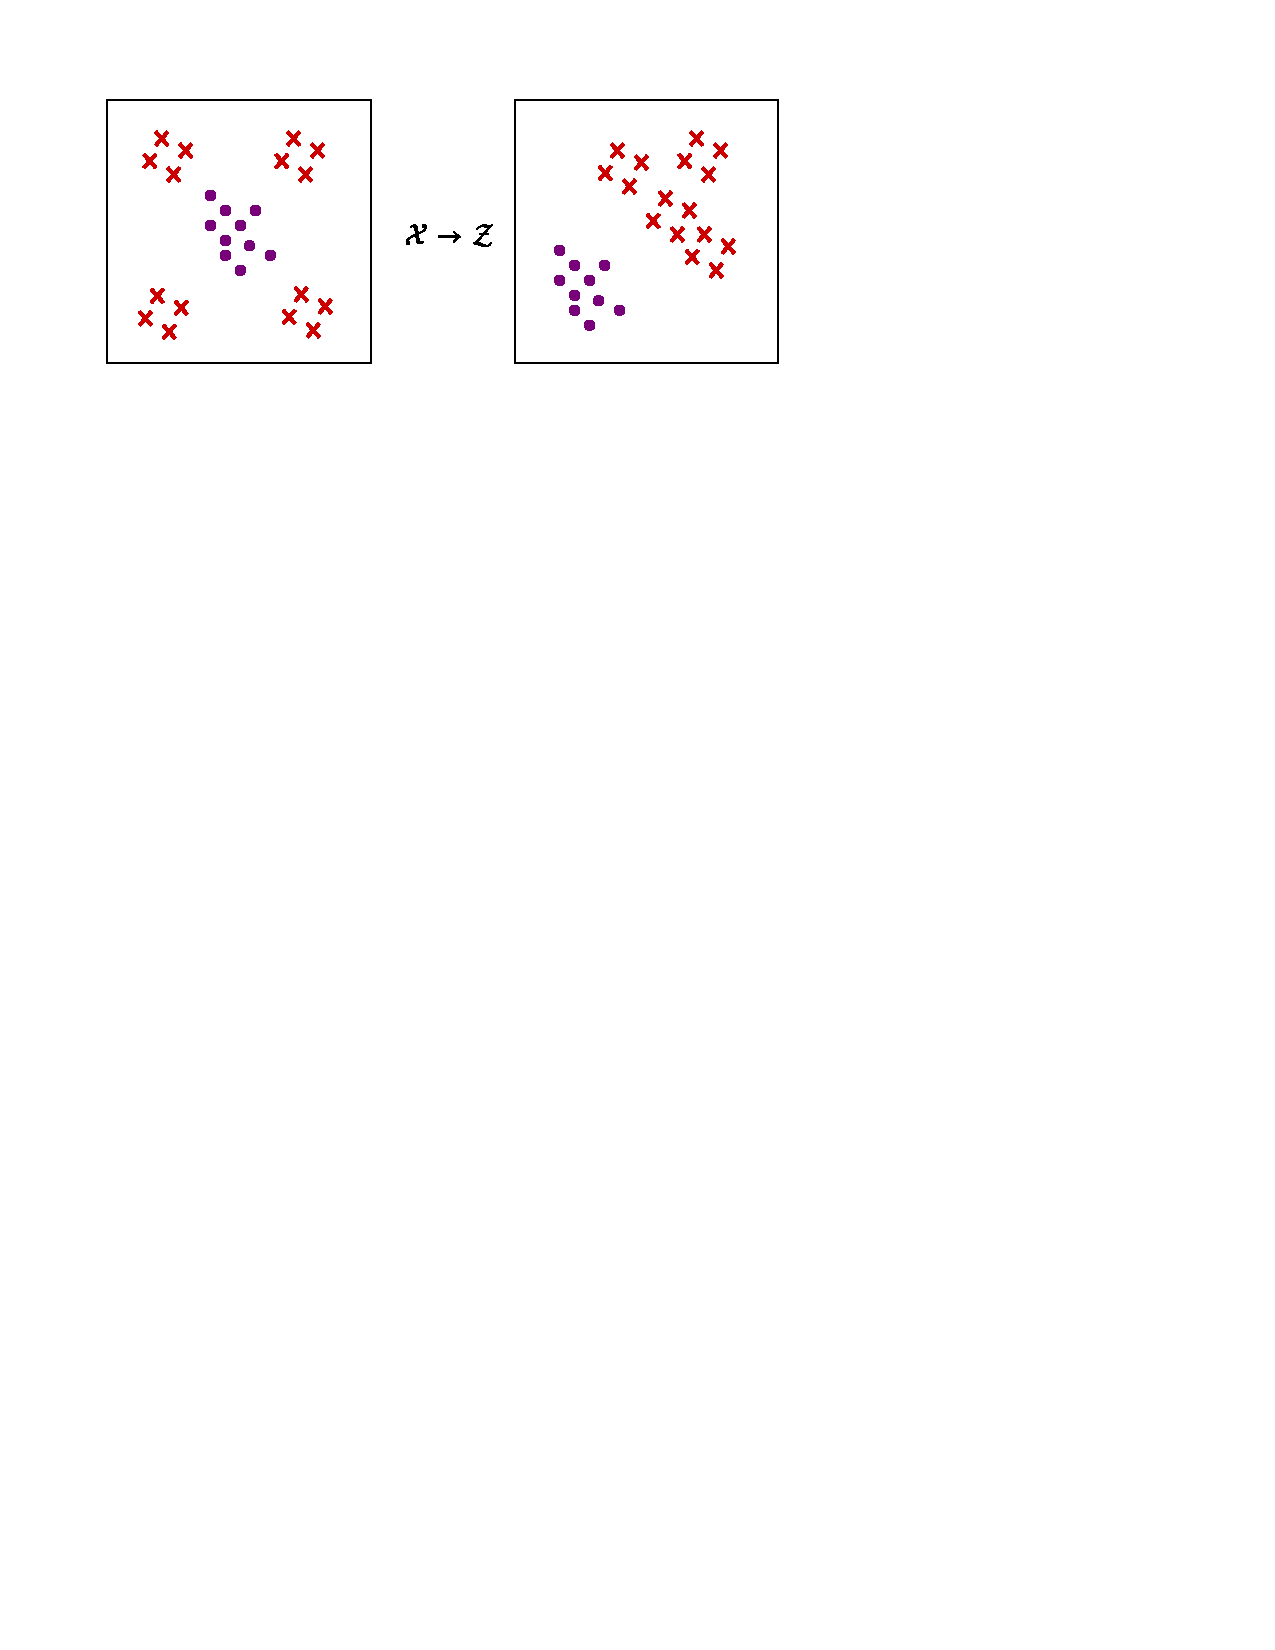
\includegraphics[width=\textwidth]{SVM07}
%\end{figure}
%\end{frame}

\begin{frame}{Solution}
\begin{itemize}
\item Since the data is linear separable, we can use a linear SVM.
\item By inspection, it should be obvious that there are three support vectors.
\begin{figure}
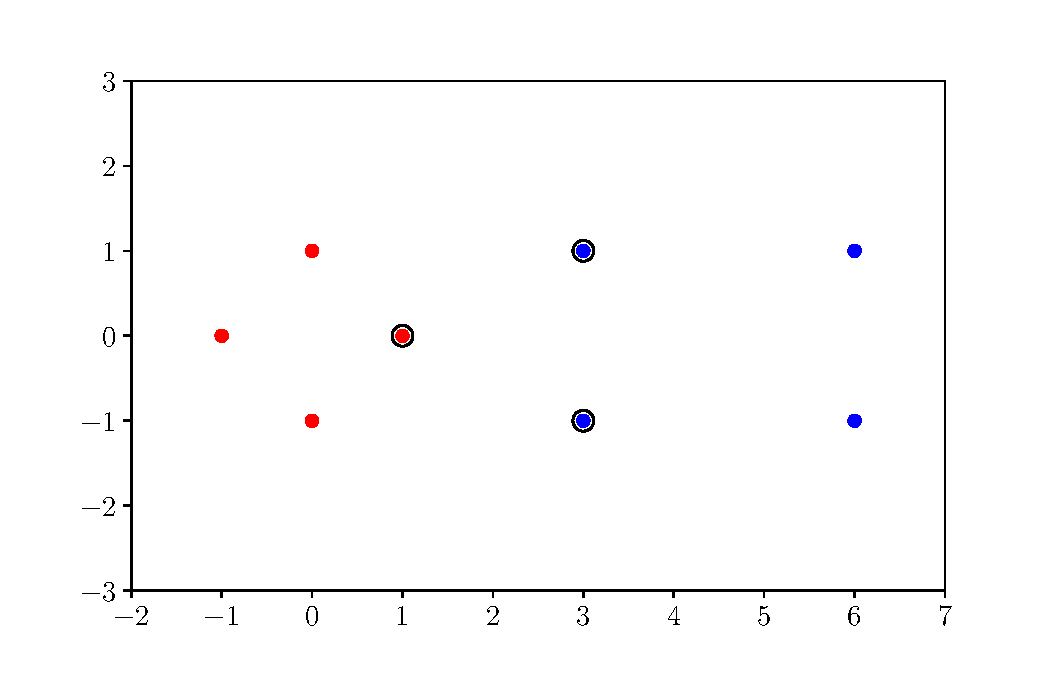
\includegraphics[scale=0.45]{data7.pdf}
\end{figure}
\end{itemize}
\end{frame}
\begin{frame}{QP hand us $\alpha$}
\begin{figure}
\includegraphics[width=\textwidth]{SVM08}
\end{figure}
\end{frame}


\begin{frame}{Support vectors}
\begin{figure}
\includegraphics[width=\textwidth]{SVM09}
\end{figure}
\end{frame}

\begin{frame}{${\rm z}$ instead of ${\rm x}$}
\begin{figure}
\includegraphics[width=\textwidth]{SVM20}
\end{figure}
\end{frame}

\begin{frame}{"Support vectors" in $\mathcal{X}$ space}
\begin{figure}
\includegraphics[width=\textwidth]{SVM21}
\end{figure}
\end{frame}

\begin{frame}{Kernel Trick: What do we need from the $\mathcal{Z}$ space?}
\begin{figure}
\includegraphics[width=\textwidth]{SVM10}
\end{figure}
\end{frame}

\begin{frame}{Generalized inner product}
\begin{figure}
\includegraphics[width=\textwidth]{SVM11}
\end{figure}
\end{frame}

\begin{frame}{The trick}
\begin{figure}
\includegraphics[width=\textwidth]{SVM12}
\end{figure}
\end{frame}

\begin{frame}{The polynomial kernel}
\begin{figure}
\includegraphics[width=\textwidth]{SVM13}
\end{figure}
\end{frame}

\begin{frame}{We only need $\mathcal{Z}$ to exist!}
\begin{figure}
\includegraphics[width=\textwidth]{SVM14}
\end{figure}
\end{frame}

\begin{frame}{This kernel in action}
\begin{figure}
\includegraphics[width=\textwidth]{SVM15}
\end{figure}
\end{frame}

\begin{frame}{Kernel formulation of SVM}
\begin{figure}
\includegraphics[width=\textwidth]{SVM16}
\end{figure}
\end{frame}

\begin{frame}{The final hypothesis}
\begin{figure}
\includegraphics[width=\textwidth]{SVM17}
\end{figure}
\end{frame}

\begin{frame}{How do we know that $\mathcal{Z}$ exists...}
\begin{figure}
\includegraphics[width=\textwidth]{SVM18}
\end{figure}
\end{frame}

\begin{frame}{Design your own kernel}
\begin{figure}
\includegraphics[width=\textwidth]{SVM19}
\end{figure}
\end{frame}

\begin{frame}{Two types of non-separable}
\begin{figure}
\includegraphics[width=\textwidth]{SVM22}
\end{figure}
\end{frame}

\begin{frame}{Error measure}
\begin{figure}
\includegraphics[width=\textwidth]{SVM23}
\end{figure}
\end{frame}

\begin{frame}{The new optimization}
\begin{figure}
\includegraphics[width=\textwidth]{SVM24}
\end{figure}
\end{frame}

\begin{frame}{Lagrange formulation}
\begin{figure}
\includegraphics[width=\textwidth]{SVM25}
\end{figure}
\end{frame}

\begin{frame}{and the solution is ...}
\begin{figure}
\includegraphics[width=\textwidth]{SVM26}
\end{figure}
\end{frame}

\begin{frame}{Types of support vectors}
\begin{figure}
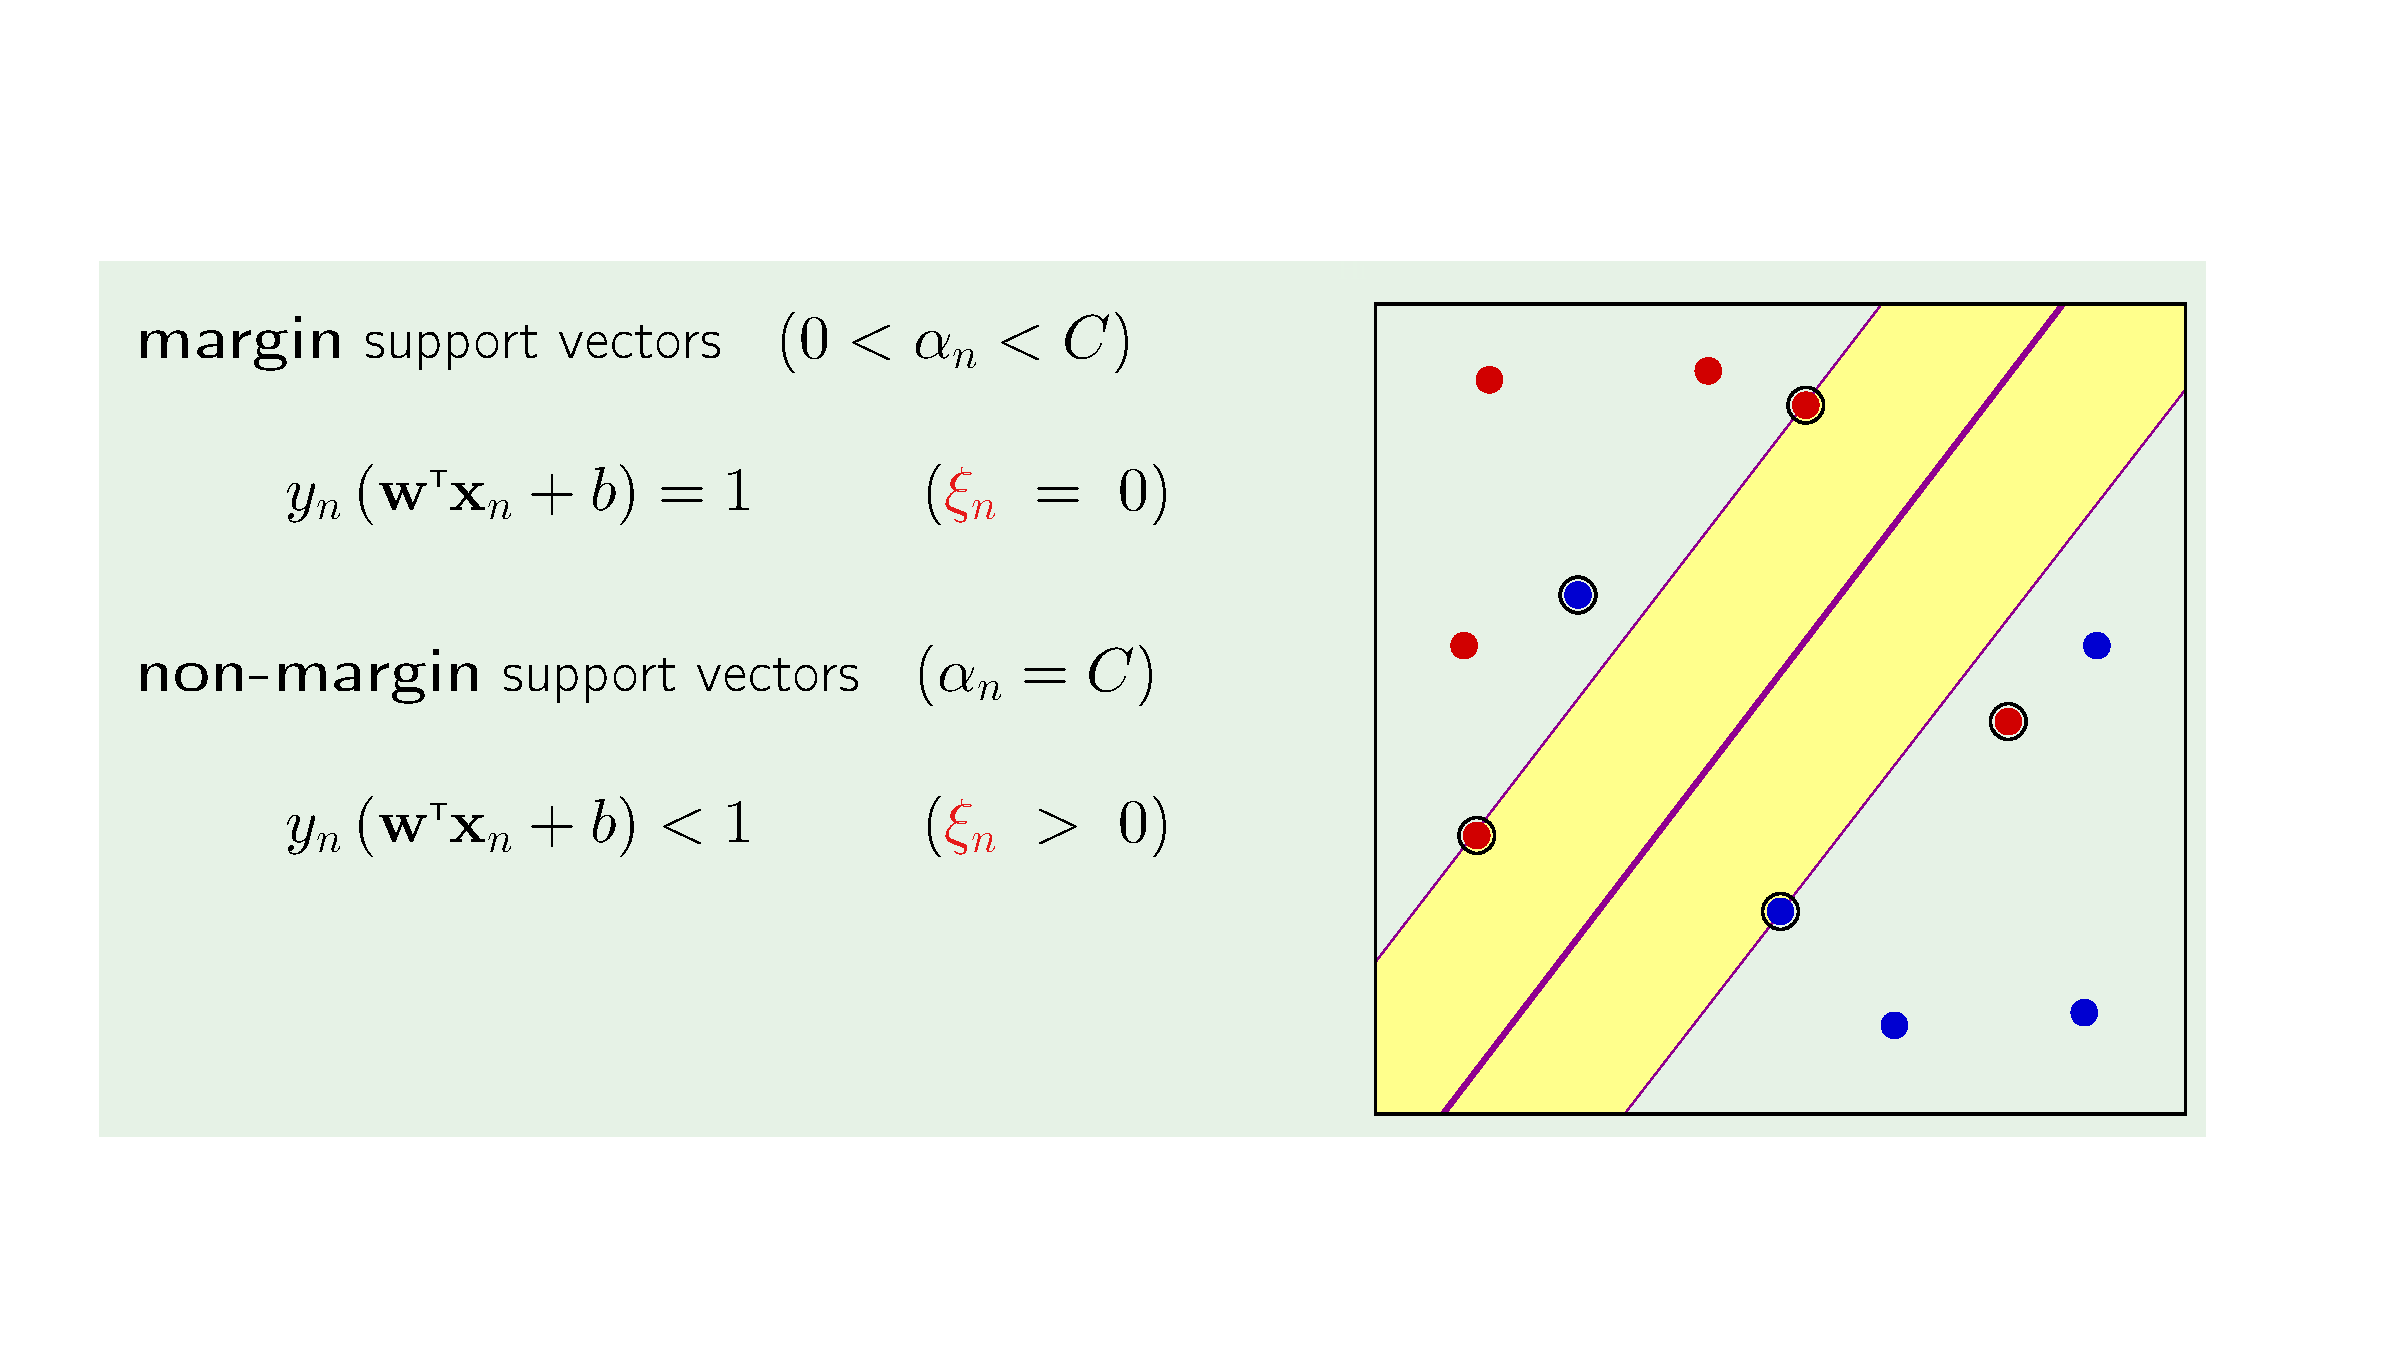
\includegraphics[width=\textwidth]{SVM27}
\end{figure}
\end{frame}

\begin{frame}{Two technical observations}
\begin{figure}
\includegraphics[width=\textwidth]{SVM28}
\end{figure}
\end{frame}

\section{References}
\subsection{}
\begin{frame}[allowframebreaks]{References}
\linespread{1}
\footnotesize
\printbibliography[heading=none]
\end{frame}
{
\setbeamertemplate{logo}{}
\makeatletter
\setbeamertemplate{footline}{
        \leavevmode%
  
  % First line.
  \hbox{%
  \begin{beamercolorbox}[wd=.2\paperwidth,ht=\beamer@decolines@lineup,dp=0pt]{}%
  \end{beamercolorbox}%
  \begin{beamercolorbox}[wd=.8\paperwidth,ht=\beamer@decolines@lineup,dp=0pt]{lineup}%
  \end{beamercolorbox}%
  } %
  % Second line.
  \hbox{%
  \begin{beamercolorbox}[wd=\paperwidth,ht=\beamer@decolines@linemid,dp=0pt]{linemid}%
  \end{beamercolorbox}%
  } %
  % Third line.
  \hbox{%
  \begin{beamercolorbox}[wd=.1\paperwidth,ht=\beamer@decolines@linebottom,dp=0pt]{}%
  \end{beamercolorbox}%
  \begin{beamercolorbox}[wd=.9\paperwidth,ht=\beamer@decolines@linebottom,dp=0pt]{linebottom}%
  \end{beamercolorbox}%
  }%
        }
\makeatother

\begin{frame}
\centering
\includegraphics[width=0.4\paperwidth]{queries.jpg}\\
\includegraphics[width=0.5\paperwidth]{thank_you.png}
\end{frame}
}
